%% Basierend auf einer TeXnicCenter-Vorlage von Tino Weinkauf.
%%%%%%%%%%%%%%%%%%%%%%%%%%%%%%%%%%%%%%%%%%%%%%%%%%%%%%%%%%%%%%
\documentclass[a4paper,oneside,12pt]{report}
% Alternative Optionen:
%	Papiergröße: a4paper / a5paper / b5paper / letterpaper / legalpaper / executivepaper
% Duplex: oneside / twoside
% Grundlegende Fontgrößen: 10pt / 11pt / 12pt

%%% Pakete
%% Spracheinstellungen & Codierung
\usepackage[ngerman]{babel} %%Für deutsche Lokalisierung und Silbentrennung
\usepackage[utf8]{inputenc}  %%Erlaubt die Verwendung von UTF-8 Kodierung
\usepackage[T1]{fontenc} %%Verbessert die Schriftkodierung für europäische/sprachspezifische Zeichen
%%Layout
%\usepackage{lmodern}  %%Lädt die "Latin Modern" Schriftfamilie für eine bessere Darstellung
\usepackage[scaled]{helvet} % Lädt die Helvetica Schriftart
\usepackage{titling}  %%Bietet zusätzliche Anpassungsmöglichkeiten für den Titel und die Titelseite
\usepackage{setspace} %%Zur Einstellung des Zeilenabstands (erneut aufgeführt, möglicherweise ein Versehen)
\usepackage{a4wide} %%Kleinere Seitenränder = mehr Text pro Zeile.
\usepackage{fancyhdr} %%Fancy Kopf- und Fußzeilen
\usepackage{titlesec} %%Zur Anpassung von Titeln und Überschriften
\usepackage{geometry} %%Zur einfachen Anpassung der Seitenränder
%%Text Design
\usepackage{color} %%Ermöglicht die Verwendung von Farben
\usepackage{xcolor} %%Definiert Farben und bietet vielfältige Farboptionen
\usepackage{soul}  %%Bietet Möglichkeiten zum Unterstreichen, Durchstreichen und Hervorheben von Text
\usepackage{hyperref}  %%Zur Erstellung von Hyperlinks innerhalb des Dokuments oder zu externen Quellen
\usepackage{listings} %%Zur Einbindung von Programmcode mit Syntaxhervorhebung
%% Grafik
\usepackage{float} %%Bietet erweiterte Möglichkeiten zur Positionierung von Bildern und Tabellen
\usepackage[export]{adjustbox} %%Erweitert Grafikoptionen, einschließlich Rahmen und Skalierung
\usepackage{graphicx} %%Zum Laden von Grafiken
%\usepackage{subfig} %%Teilabbildungen in einer Abbildung
%% Mathe
%\usepackage{amsmath} %%Bietet umfangreiche Funktionen zur Darstellung mathematischer Formeln
%\usepackage{amsthm} %%Zur Definition und Formatierung von Theoremen, Definitionen etc.
%\usepackage{amsfonts}  %%Stellt zusätzliche mathematische Schriftarten und Symbole bereit
%% Tabellen
\usepackage{tabularx}  %%Erweitert Tabellenfunktionen, erlaubt Tabellen mit automatischer Breitenanpassung
\usepackage{xltabular} %Kombiniert 'longtable' und 'tabularx', für lange Tabellen mit automatischer Breitenanpassung
%\usepackage{longtable} %%Für Tabellen, die eine Seite überschreiten
%\usepackage{tabu} %%Bietet eine modernere und flexiblere Schnittstelle für Tabellen
%% Querformat
\usepackage{lscape} %%Ermöglicht Seiten im Querformat innerhalb eines ansonsten hochformatigen Dokuments
\usepackage{pdflscape} %%Verbessert 'lscape' durch Rotation der Seiten im PDF für bessere Bildschirmdarstellung
%% Imports
\usepackage{import} %%Vereinfacht das Einbinden von Dateien aus unterschiedlichen Verzeichnissen
\usepackage{pdfpages} %%Zum Einfügen von externen PDF-Seiten in das Dokument
%%Verzeichnisse
\usepackage[toc,page,title]{appendix}
\usepackage{etoolbox}
\appto\appendix{\addtocontents{toc}{\protect\setcounter{tocdepth}{0}}}
\appto\listoffigures{\addtocontents{lof}{\protect\setcounter{tocdepth}{1}}}
\appto\listoftables{\addtocontents{lot}{\protect\setcounter{tocdepth}{1}}}

%%% Einstellungen
%% Seitenränder
\geometry{
    a4paper,
    top=2.5cm,
    left=2.5cm,
    right=2cm,
    bottom=4cm,
    headheight=1.25cm,
    footskip=1.1cm
}

%% Kopf- und Fußzeilen
\fancypagestyle{plain}{
    \fancyhf{} % Löscht die aktuelle Kopf- und Fußzeile
    \renewcommand{\headrulewidth}{1pt} % Entfernt die Linie unter der Kopfzeile
    \renewcommand{\footrulewidth}{1pt} % Entfernt die Linie über der Fußzeile

    \fancyhead[L]{\leftmark} % Links: Kapitelname
    \fancyhead[C]{} % Zentriert: leer
    \fancyhead[R]{CKi ein CNN-Model in C++} % Rechts:  Dokumenttitel

    \fancyfoot[L]{Kantonsschule Frauenfeld} % Links: Name
    \fancyfoot[C]{} % Zentriert: leer
    \fancyfoot[R]{\thepage} % Rechts: Seitenzahl
}
\pagestyle{empty} %Keine Kopf-/Fusszeilen auf den ersten Seiten

%% Überschriften
\titleformat{\chapter}[hang]{\bfseries\Large}{\thechapter}{16pt}{\Large}[{\vspace{8pt}}]
\titleformat{\section}[hang]{\bfseries\large}{\thesection}{14pt}{\large}[{\vspace{7pt}}]
\titleformat{\subsection}[hang]{\bfseries\normalsize}{\thesubsection}{12pt}{\normalsize}[{\vspace{6pt}}]
\titleformat{\subsubsection}[hang]{\normalsize}{\thesubsubsection}{12pt}{\normalsize}[{\vspace{6pt}}]

%% Standardtext Einstellungen
%\renewcommand{\normalsize}{\fontsize{11pt}{12pt}\selectfont} % Setzt die Schriftgröße auf 11pt
\renewcommand*\familydefault{\sfdefault} % Setzt die Standard-Schriftart auf Sans-Serif (Helvetica/Arial)

%% Zeilenabstand
\setstretch{1.5}

%% Code
%from chatgpt
\definecolor{codegreen}{rgb}{0,0.6,0}
\definecolor{codegray}{rgb}{0.5,0.5,0.5}
\definecolor{codepurple}{rgb}{0.58,0,0.82}
\definecolor{backcolour}{rgb}{0.95,0.95,0.92}
\lstset{
    basicstyle=\footnotesize\sffamily\color{black},
    commentstyle=\color{codegray},
    frame=single,
    numbers=left,
    numbersep=5pt,
    numberstyle=\tiny\color{codegray},
    %keywordstyle=\color{blue}\bfseries,
    keywordstyle=\emph{},
    showspaces=false,
    showstringspaces=false,
    stringstyle=\color{codepurple},
    tabsize=2,
    backgroundcolor=\color{backcolour},
    morekeywords={include, printf, std::vector}, % C++ keywords to highlight
    language=C++, % This ensures we are using C++ syntax highlighting
    breaklines=true, % This will automatically break long lines
    prebreak=\raisebox{0ex}[0ex][0ex]{\ensuremath{\hookleftarrow}}, % Adds a hook arrow at the end of the line indicating a break
    postbreak=\raisebox{0ex}[0ex][0ex]{\ensuremath{\hookrightarrow}\space}, % Adds a hook arrow at the start of the next line
}

%%Grafik
\graphicspath{ {./images/} } %%Ordner, in dem die Grafiken gesucht werden
% Beachten Sie:
% Die Einbindung einer Grafik erfolgt mit \includegraphics{Dateiname}
% bzw. über den Dialog im Einfügen-Menü.
%
% Im Modus "LaTeX => PDF" können Sie u.a. folgende Grafikformate verwenden:
%   .jpg  .png  .pdf  .mps
%
% In den Modi "LaTeX => DVI", "LaTeX => PS" und "LaTeX => PS => PDF"
% können Sie u.a. folgende Grafikformate verwenden:
%   .eps  .ps  .bmp  .pict  .pntg

%% Deckblatt
\title{CKi ein CNN-Model in C++}
\author{Simeon Stix}
\date{\today}
\renewcommand{\maketitle}{
\begin{titlepage}
    \begin{center}
        \vspace*{1cm}
        
        \Huge
        \textbf{\thetitle}
        
        \vspace{0.5cm}
        \Large
        by \theauthor
        
        \vspace{1.5cm}
        
        \today
        
        \vfill
        
        Version: 2.1
        
        \vspace{1cm}
        
        Betreuer: Sven Nüesch
        
    \end{center}
\end{titlepage}
}

\begin{document}

\maketitle

\pagestyle{plain} %%Ab hier die Kopf-/Fusszeilen: headings / fancy / ...

%% Inhaltsverzeichnis 
\tableofcontents %Inhaltsverzeichnis
\setcounter{secnumdepth}{4} %Setzung der Nummerierungstiefe
\setcounter{tocdepth}{3} %Setung der Anzeige der Nummerierungstiefe im Inhaltsverzeichnis
%\cleardoublepage %Das erste Kapitel soll auf einer ungeraden Seite beginnen.

%% Hauptteil
%%Analyse
\chapter{Analyse}
\label{sec:Analyse}
\section{Aufgabenstellung}
\label{sec:AnalyseAufgabenstellung}
Die Aufgabe, die sich das Projekt CKi stellt, ist die Wissenserweiterung des Entwicklers. Dabei wird ein Programm geschrieben, welches einzelnen handgeschriebenen Ziffern erkennen kann. Dies geschieht mittels KI. Dabei wird die KI komplett vom Entwickler geschrieben. Da keine modernen externen Grundlagen verwendet werden, wird das Produkt, das Programm, nicht die Geschwindigkeit einer modernen KI erreichen. Dies spielt jedoch keine Rolle, da dieses Projekt nicht wegen des Endprodukts durchgeführt wird.

\section{Zielgruppe}
\label{sec:AnalyseZielgruppe}
Das Projekt CKi ist als solches nicht ausgelegt, einem realen Anwendungszweck zu entsprechen oder eine Lösung oder einen Lösungsansatz für einen solchen zu bieten. Diesbezüglich liegt der einzige Nutzen von CKi nicht in dessen Produkt, sondern nur im Wissensgewinn und Verständnis gewinn für den Entwickler in den Bereichen der künstlichen Intelligent oder genauer im Bereich des maschinellen Lernens mit einem \textit{Convolutional Neural Network}, der Realisation von Anwendungen mit C++ und dessen Möglichkeiten Hardware direkt in die programminternen Abläufe einzubinden. Somit richtet sich CKi nicht nach dem Grundsatz ein bestmögliches nutzbares Produkt zu sein, sondern lediglich nach dem grössten Wissensgewinn für den Entwickler. Nach diesem Grundsatz ist die resultierende Zielgruppe der Entwickler und vereint so multiple Rollen des Projektes CKi in einer Person.

\section{Anforderungen}
\label{sec:AnalyseAnforderungen}

\subsection{Must-haves}
\label{sec:AnalyseMustHaveS}
Die Must-haves wurden aus dem Themenblatt, welches am 15.09.2023 bei Walter Schnyder eingereicht wurde, übernommen und mit weiterführenden Elaborationen versehen.

\begin{itemize}
\item 
Rückgabe in Prozentwerten, die die Wahrscheinlichkeit der Übereinstimmung mit dem digitalen Gegenstück der handgeschriebenen Zahl abbildet. "Welche Zahl wurde (vermutlich) aufgeschrieben?"
\subparagraph{}
\textbf{Erläuterung:}
Da ein simples neuronales Netzwerk für maschinelles Lernen durch ein "Netz" aus Knotenpunkten gebaut wird und jeder dieser Knotenpunkte, auch die Knotenpunkte, welche bei einem solchen neuralen Netzwerk als Endschnittstellen fungieren, einzeln berechnet werden, erhält man, bei Anwendungsfall von CKi, eine multiple Anzahl von Prozentzahlen, welche zur Interpretation es gelieferten Endergebnisses verwendet werden können. Diese Rückgabe der einzelnen Prozentwerte erfolgt zum Beginn über eine Konsolenausgabe. Diese wird später, wie in \textit{"Nice-to-haves"} unter GUI erläutert, in ein grafisches Nutzerinterface integriert und zu diesem Zeitpunkt evtl. auch interpretiert (wobei die einzelnen Prozentwerte weiterhin einsichtig bleiben sollten).

\item CNN-Algorithmus (trainiert auf Zahlenwert)
\subparagraph{}
\textbf{Erläuterung:}
Ein CNN-Algorithmus oder auch Convolutional Neural Network wird beim maschinellen Lernen oft bei der Interpretation von Bildern genutzt. Dabei wird das Bild in kleinere Abschnitte unterteilt und „einzeln“ an den gehirnähnlich aufgebauten Algorithmus weitergegeben.
\begin{figure}[H]
\centering
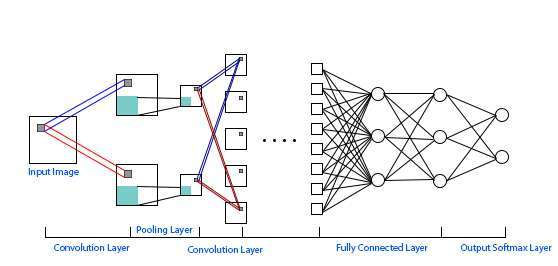
\includegraphics[scale=0.5]{CNN-model-with-several-convolution-and-pooling-layers-performed-alternately-combined.jpeg}
%von https://www.researchgate.net/publication/309751512/figure/fig1/AS:503017750437888@1496940185276/CNN-model-with-several-convolution-and-pooling-layers-performed-alternately-combined.png
\caption{CNN Model Aufbau Grafik}
\label{fig:AnalyseCNN-model-with-several-convolution-and-pooling-layers-performed-alternately-combined}
\end{figure}
Im Projekt CKi wird dieser wie im Themenblatt beschrieben mit Bild von einzelnen handgeschriebenen Ziffern trainiert.

\item Nutzer-Input → Nutzer darf eine Zahl zeichnen
\subparagraph{}
\textbf{Erläuterung:}
Ein solches CNN-Model zu erbauen und zu trainieren ist zwar die Grundlage für dieses Must-have, jedoch sollte das Produkt auch erprob bar sein. Diesbezüglich muss der Nutzer in der Lage sein, eine handschriftliche Ziffer an das neurale Netzwerk zu liefern. Hierbei ist die minimale Anforderung, dass der Nutzer in einer anderweitigen Applikation ein solches Bild erstellt hat und es nun interpretieren lassen kann. Wie in Nice-to-haves unter GUI beschreiben, wird diese Eingabemöglichkeit (eine Ziffer zu zeichnen oder eine schon vorhandene grafische Abbildung zu verwenden) in einem weiteren Entwicklungsschritt direkt in die grafische Nutzeroberfläche der Applikation integriert.

\end{itemize}

\subsection{Nice-to-haves}
\label{sec:AnalyseNiceToHaveS}
Die Nice-to-haves wurden aus dem Themenblatt, welches am 15.09.2023 bei Walter Schnyder eingereicht wurde, übernommen und mit weiterführenden Elaborationen versehen. Zudem behalte ich mir als Verfasser dieses Dokumentes, als Entwickler des Projektes CKi und als Zielgruppe des Projektes CKi vor, diese Liste in gegebene Falle zu erweitern.

\begin{itemize}
\item GUI
\subparagraph{}
\textbf{Erläuterung:}
Ein GUI (oder auch Graphical User-Interface) ist die grafische Nutzeroberfläche der Applikation. Da die Applikation primär dem Wissensgewinn gewidmet ist und dementsprechend nicht für den Nutzer optimiert wird, hat eine solche Erweiterung nur eine geringe Priorität. Diese Nutzeroberfläche wird selbst bei der Umsetzung in einer möglichst simplen Form gehalten. Dabei sollte es folgende Bestandteile beinhalten:
\begin{itemize}
\item Eine Möglichkeit für den Nutzer eine anderweitig gezeichnete Ziffer interpretieren zu lassen
\item Eine Möglichkeit für den Nutzer eine Ziffer zu zeichnen.
\item Eine weiter-interpretierte Ausgabe der Interpretation des CNN.
\item Eine Ausgabe des nicht interpretierten Prozentwertes der Interpretation des CNN.
\end{itemize}
Bis zu dem Punkt, wo ein GUI realisiert wurde und in den Einsatz gestellt wird, sind nicht alle dieser Funktionen über die Konsole (das Interface zum Programm, welches vor dem GUI zum Einsatz kommt) verfügbar.

\item GPU als Berechnungsplattform nutzen
\subparagraph{}
\textbf{Erläuterung:}
Die CPU in jedem Computer ist eine sehr „fokussierte“ Hardware, immer nur einen einzelnen Prozess kann diese berechnen. Dies ist für ein neuronales Netzwerk, welche Hunderte oder Tausende von Knotenpunkten in seinem Netzwerk hat und alle einzeln berechnet werden müssen, äusserst hinderlich. Die dezidierte Grafikkarte, wenn vorhanden, kann diesem Geschwindigkeitsverlust nachhelfen, da eine solche GPU in der Lage ist, tausende Berechnungen gleichzeitig zu tätigen.
Da im Projekt mit C++, einer Hardware-nahen Programmiersprache, gearbeitet wird, kann eine Anbindung an das Rechenpotential der GPU erreicht werden. Da dies jedoch ein äusserst schwieriger Prozess ist, sich diese Anbindung bei den unterschiedlichen Herstellern von GPUs unterscheiden kann und ich notwendig um ein funktionierendes CNN zu erstellen, wurde diese Optimierung als nicht notwendig eingestuft.
\end{itemize}

\subsection{Use Cases}
\label{sec:AnalyseUseCases}
Die hier aufgelisteten Use Cases entsprechen den Use Cases nach den Must-haves und sind diesbezüglich ohne die grafische Nutzeroberfläche. Dies kann dazu führen, dass ein endgültiges Produkt nicht mehr kohärent zu den Use Cases steht. Im Allgemeinen sollte aber selbst eine solche Inkohärenz nicht in extremer Weise auftreten, da die Bedienung der Applikation als Konsole als auch als grafische Oberfläche in ähnlicher Weise auftreten sollte.

\begin{landscape}
\begin{xltabular}{\linewidth}{|X|X|X|X|X|X|X|}
\hline
Nummer & Name & Akteur  & Ablauf & Nachbedingungen & Ausnahmen & Anmerkungen
\\\hline
1 & 
Interpretation & 
Nutzer, CNN  & 
Siehe Ablaufdiagramm "Interpretation" & 
Der Nutzer sollte in der Konsole eine Auflistung aller möglichen Ziffern (0-9) und deren entsprechenden Wahrscheinlichkeit sehen. Zudem kann der Nutzer auch die kongruierende Zahl zur höchsten Möglichkeit auf einer speziellen Zeile in der Konsole ablesen. & 
Bei der Interpretation von Nutzer-eigenen Abbildungen kann es zu multiplexen Fehlern kommen. Diese reichen von falschen Dateikodierung zu falscher Auflösung. Aufgrund dieser mannigfaltigen Möglichkeiten zu Fehlern können diese nicht alle hier erläutert werden. Eine Auflistung aller Fehler ist in der Dokumentation unter "\textit{Fehler}" zu finden. & 
Offiziell ist zwar Training keine Vorbedingung zu Testet, jedoch macht die Anwendung der Applikation keinen Sinn, wenn man nicht erwarten kann, dass man ein realistisches oder sinnvolles Ergebnis erhält.

\\\hline
2 &
Training & 
Nutzer, CNN  & 
Siehe Ablaufdiagramm "Training" & 
Der Nutzer erhält nach der Beendigung der Schulung des CNN-Models eine kurze Benachrichtigung, dass das Training abgeschlossen ist. Zudem erhält der Nutzer nach jedem einzelnen Datensatz den Output, dass nun x von y Datensätzen bearbeitet wurden.  & 
Hierbei kann es zu zwei Fehlern kommen. Dabei handelt es sich beides um Fehler bei der Datenbank. Der erste ist ein Fehler, wenn die benötigten "Tabellen" in der Datenbank nicht stimmig mit den Erwartungen sind und der andere, wenn keine Daten in der Datenbank zu finden sind. Für die genauen Fehlercodes ist die Dokumentation unter "\textit{Fehler}" zu kontaktieren. &
\\\hline
3 & 
Testen & 
Nutzer, CNN & 
Siehe Ablaufdiagramm "Testen" & 
Der Nutzer findet nach jedem Datensatz in der Test-Datenbank eine simple Gegenüberstellung der richtigen und der falschen interpretierten Ziffern. Diese weiterzuverarbeiten, ist dem Nutzer überlassen. Neben der Gegenüberstellung erhält der Nutzer auch die Benachrichtigung, dass nun x von y Datensätzen bearbeitet wurden. & 
Hier kann es zu zwei Fehlern kommen. Dabei handelt es sich beides um Fehler bei der Datenbank. Der erste ist ein Fehler, wenn die benötigten "Tabellen" in der Datenbank nicht stimmig mit den Erwartungen sind und der andere, wenn keine Daten in der Datenbank zu finden sind. Für die genauen Fehlercodes ist die Dokumentation unter "\textit{Fehler}" zu kontaktieren. & 
Bei den Testdaten würde es evtl. Sinn machen, die einzelnen Konsolen Outputs auch in einer CSV-Datei festzuhalten, wobei dies mit Pipes in der Konsole dem Nutzer bereits offensteht.  
Offiziell ist zwar Training keine Vorbedingung zu Testet, jedoch macht das Testen nur begrenze Sinn, wenn es noch nichts gibt, was sich zu testen lohnt. 
\\\hline
\end{xltabular}
\label{tab:AnalyseUseCases}
\end{landscape}

\subsection{Use Case Diagramme}
\label{sec:AnalyseUseCaseDiagramme}
\begin{figure}[H]
\centering
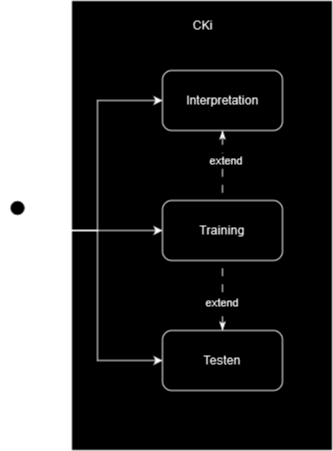
\includegraphics[height=0.5\paperheight]{usecase.png}
\caption{Use-Case-Diagramm}
\label{fig:analyseusecase}
\end{figure}

\subsection{Ablaufdiagramme}
\label{sec:AnalyseAblaufdiagramme}

\subsubsection{Interpretation}
\label{sec:AnalyseInterpretation}
\begin{figure}[H]
\centering
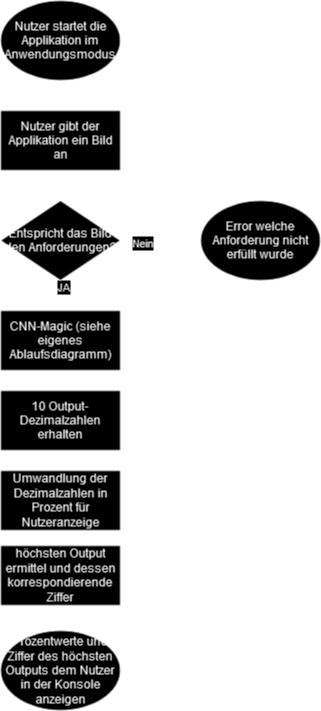
\includegraphics[height=0.5\paperheight]{ablauf-interpretation.png}
\caption{Ablaufdiagramm für die Interpretation von Nutzer-gelieferten Einzelbildern}
\label{fig:analyseablauf-interpretation}
\end{figure}


\subsubsection{Training}
\label{sec:AnalyseTraining}
\begin{figure}[H]
\centering
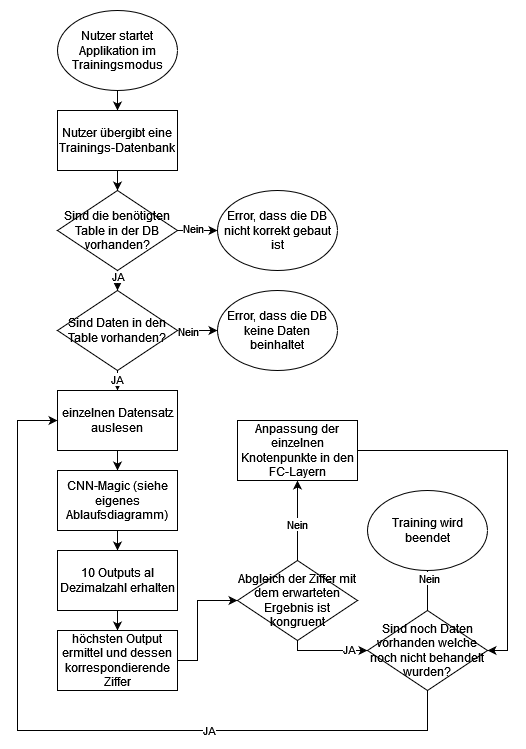
\includegraphics[height=0.5\paperheight]{ablauf-training.png}
\caption{Ablaufdiagramm vom Training des CNN}
\label{fig:analyseablauf-training}
\end{figure}


\subsubsection{Testen}
\label{sec:AnalyseTesten}
\begin{figure}[H]
\centering
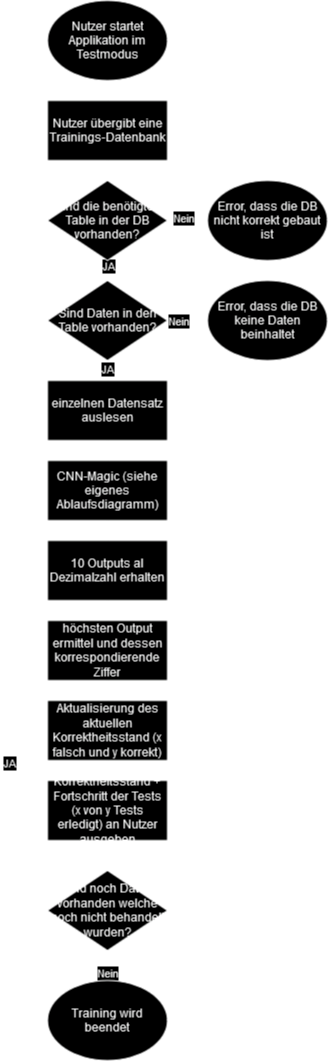
\includegraphics[height=0.5\paperheight]{ablauf-testen.png}
\caption{Ablaufdiagramm von einem Test des CNN}
\label{fig:analyseablauf-testen}
\end{figure}


\subsubsection{CNN-Magic}
\label{sec:AnalyseCNN-Magic}
\begin{figure}[H]
\centering
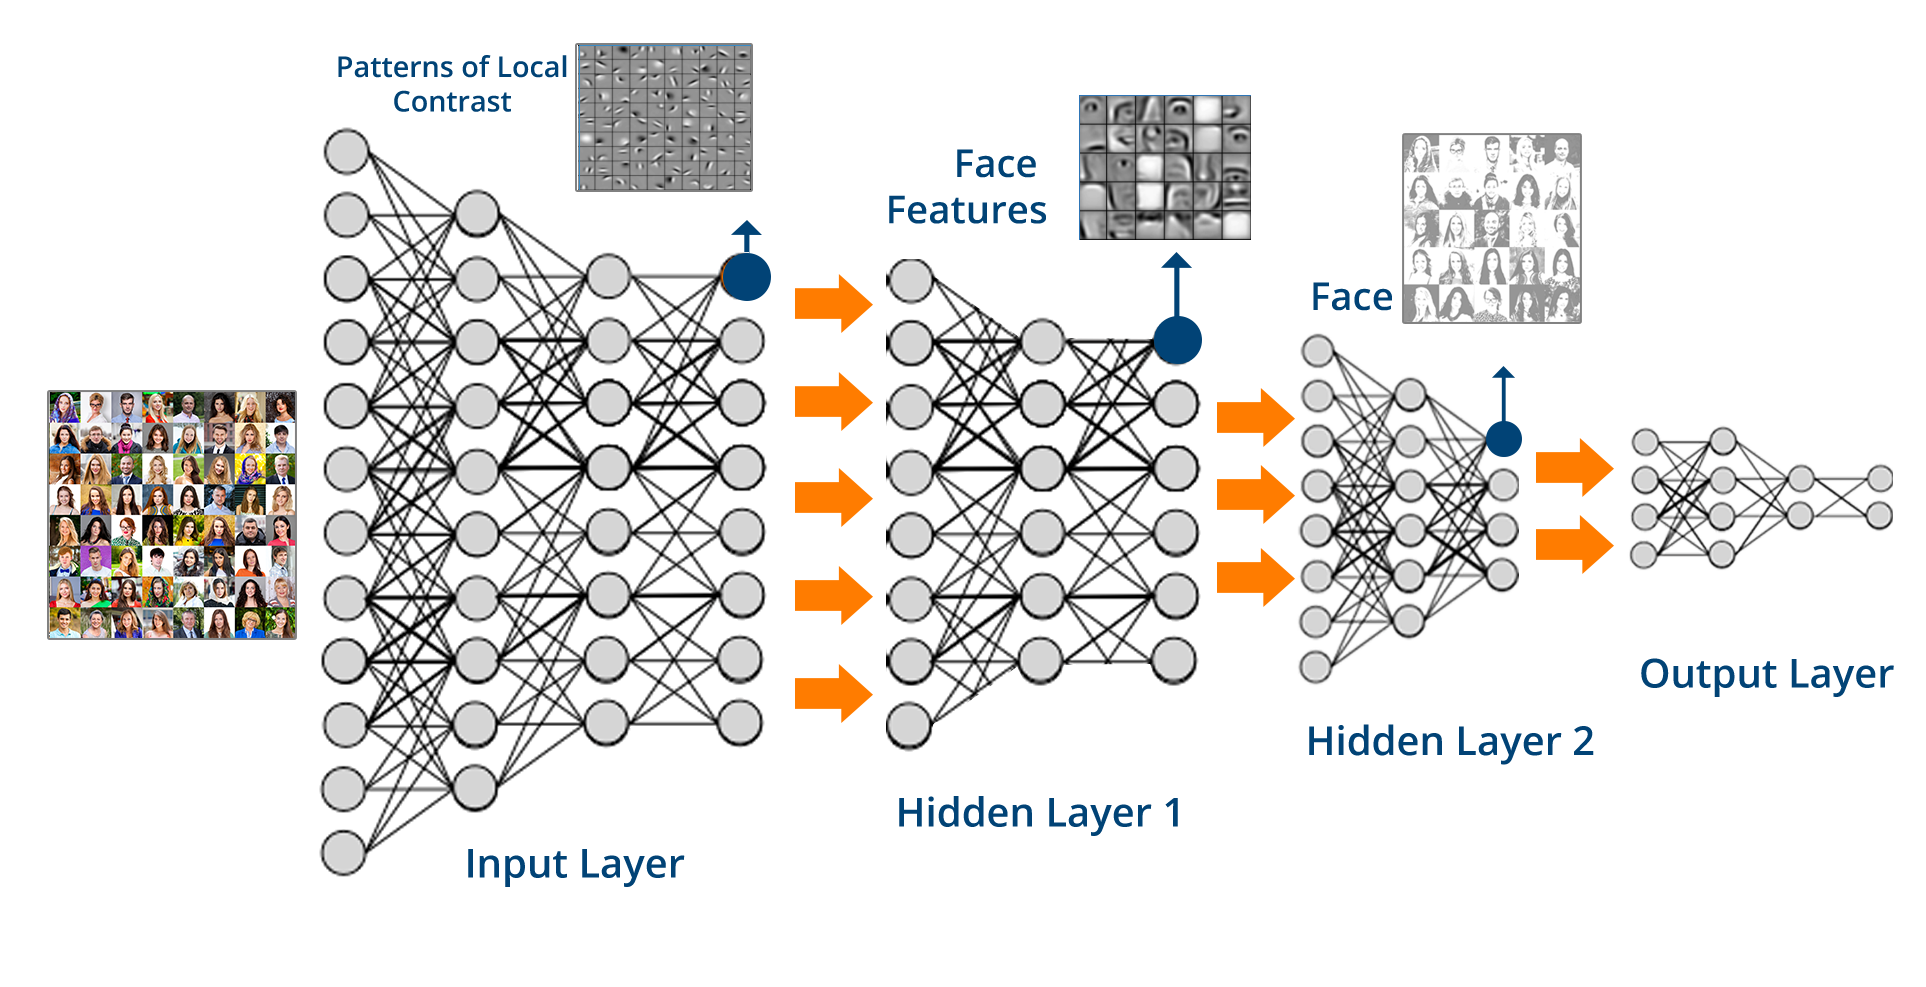
\includegraphics[width=\linewidth]{1 RXJ6tAmfN1AYLQr7p48L7w-631173908.png}
% von https://external-content.duckduckgo.com/iu/?u=https%3A%2F%2Fmiro.medium.com%2Fproxy%2F1*RXJ6tAmfN1AYLQr7p48L7w.png&f=1&nofb=1&ipt=4eb63d23b17398cd376f86942611c6a9fda3b4520fc8eb09e736d7f19f0d276d&ipo=images
\caption{Visuelle Darstellung der Funktionsweise eines CNN}
\label{fig:analyse1RXJ6tAmfN1AYLQr7p48L7w-631173908}
\end{figure}

\section{Umsetzung}
\label{sec:AnalyseUmsetzung}
Wie im Themenblatt vom 15.09.2023 wird für die Umsetzung reines C++ verwendet.

\subsection{Entwicklungsumgebung}
\label{sec:AnalyseEntwicklungsumgebung}
Bei der Entwicklungsumgebung wird das JetBrains Produkt \textbf{CLion} zum Einsatz kommen. Dieses beinhaltet alle benötigten Funktionalitäten, die bei der Entwicklung des Produktes nötig sind. Gegebenen Falles könnte noch \textbf{SQLite Browser} zur Verwendung kommen, da dieses ein besseres (und für den Entwickler ein gewohntes) Interface zur Handhabung von lokalen Datenbanken bietet. Für die Version Control des Projektes wird lokal \textbf{Git} verwendet und zur Sicherung in der Cloud wird sowohl \textbf{GitHub} als auch \textbf{GitLab} verwendet. Die Entwicklungsumgebung mit IDE und Version Control wird primär auf dem Betriebssystem Windows verwendet. Es kann jedoch nicht garantiert sein, dass die Entwicklung nicht teilweise unter einer Distribution von Linux ablaufen wird. Hierbei sollten (evtl. abgesehen von der GUI) keine Kompatibilitätsprobleme mit sich führen. 
\subsubsection{Auflistung Versionen}
\label{sec:AnalyseDevEnvAuflistung}
\begin{itemize}
\item JetBrains Toolbox 2.1.1.18388, Windows 11, x64
\item CLion (von JetBrains Toolbox) 2023.2.2
\item Git 2.39.2.windows.1
\end{itemize}

\subsection{CNN}
\label{sec:AnalyseCNN}
\subsubsection{Grundlagen}
\label{sec:AnalyseGrundlagen}
Der Kern des CNN lässt sich in drei unterschiedliche Arten von Schichten aufteilen. Zusätzlich gibt es noch zwei zusätzliche "Hilfs-"Schichten, welche für die Ein- und Ausgaben zuständig sind. 
Die \textit{Eingabeschicht} ist eine dieser zwei erwähnten Schichten. Diese akzeptiert im Falle von CKi jeweils ein Bild von speziell definierten Grössen und nimmt, gibt jeder Pixel in Graustufen (Dies ist entscheidend, weil so der Farbwert des Pixels von drei, zwei Byte grossen Zahlen zu nur einer zwei Byte grossen Zahl reduziert wird.) als ein sogenanntes Eingabeneuron. 
Auf die Eingabeschicht folgt die \textit{Convolutional Layers} oder auch \textit{Faltungsschichten}. Diese Faltungsschichten sind einer der Schlüsselbestandteile eines CNN. Die Convolutional Layer dienen dazu, bestimmte Merkmale und Schlüsselelemente aus dem Bild zu extrahieren. Hierbei wird bei jedem der Convolutional Layer eine 
mathematische Faltungsoperationen durchführt. 
Nach den Faltungsschichten kommen die simplen \textit{Pooling-Schichten}. Bei einer Pooling-Schicht wird die Dimension eines Bildes reduziert (Downsampling). Dies kann durch zwei Arten geschehen, entweder durch Max-Pooling, dabei wird aus einer Liste von Werten nur der höchste übermittelt oder durch Durchschnitts-Pooling, wobei der Durchschnitt dieser Liste berechnet und übermittelt wird. Durch diese Datenreduktion wird Rechenleistung gespart und so das Ergebnis schneller und stabiler geliefert. 
Vor der Ausgabeschicht gibt es noch die \textit{FC Layers} oder auch \textit{Vollständig verknüpfte Schichten}. Bei diesen ist jeder Knotenpunkt mit jedem Knotenpunkt in der nächsten Schicht verbunden. Dies ist das Herz des gesamten Models. Dabei wird in jedem Knotenpunkt ein neuer Wert berechnet, um in der letzten Schicht, der \textit{Ausgabeschicht} diese in Wahrscheinlichkeit zu "konvertieren".

\subsubsection{Implementation}
\label{sec:AnalyseImplementation}
Bei der Implementation eines CNN-Models wurde für CKi der Entschluss getroffen, eine C++-Klasse für jede benötigte Art von Layer zu schreiben. Danach muss ein Grundgerüst, eine Main-Klasse realisiert werden, die alle Klassen miteinander kombiniert. Dies erleichtert es in einem späteren Schritt die grosse Umstellung von einer Konsolen-Anwendung hin zu einer grafisch passierten Anwendung (auch wenn immer noch grosse Teile der Main-Klasse ausgetauscht werden müssen.). Für die Speicherung der Berechnungswerte für die FC-Layer ist die Abwägung zu treffen, ob es sinnvoll ist, diese in einer lokalen Datenbank zu speichern oder in eine konkret hierfür entworfene Datei zu schreiben.

\subsection{Testdaten}
\label{sec:AnalyseTestdaten}
Die Testdaten für CKi können in unzähliger Ausführung auf \href{https://www.kaggle.com/}{Kaggle} gefunden werden.

\subsubsection{Speicherung}
\label{sec:AnalyseSpeicherung}
Im gegebenen Fall würde es für die Schulung, des CNN, Sinn ergeben, die einzelnen Bilder nicht über Ordner- oder Archivstrukturen zu speichern, sondern in eine oder mehrere lokale Datenbanken abzuspeichern.

\section{Abwägung des Nutzens und der Alternativen}
\label{sec:AnalyseNutzwertanalyseDerLösungsvarianten}
\subsection{Alternativen}
\label{sec:AnalyseAlternativen}
Die möglichen Alternativen zu einer kompletten Realisation eine CNN oder irgendeinem neuronalen Netzwerk in C++ ohne Bibliotheken oder Frameworks für neuronale Netze sind endlos. 
Selbst wenn man bereits bestehende Produkte begutachtet, wird man auf GitHub schnell fündig. Bei einer Suche auf GitHub mit dem Query "mnist digit recogniser" findet man nach Stand 20.10.2023 02:13 178 Repositorien (je eines in C, C++, C\#, Rust, drei in Java + Kotlin und 53 in Python).
Selbst wenn man unter dem Beschluss steht, dass man das CNN selber bauen wolle, würde man für jede beliebige Sprache eine Bibliothek oder Framework finden, die einem diese Aufgabe erleichtern würde.

\subsection{Kosten}
\label{sec:AnalyseKosten}
Bezüglich der Kosten kann das Projekt CKi nicht mit den Alternativen mithalten. C++ ist keine Sprache, in welcher man schnell ein Produkt hervorbringt. Dies belegen etliche Studien und Artikel (
\href{https://www.cs.bsu.edu/homepages/dmz/cs697/langtbl.htm}{Programming Languages Table}, 
\href{https://citeseerx.ist.psu.edu/viewdoc/download?doi=10.1.1.113.1831&rep=rep1&type=pdf}{An Empirical Comparison of Seven Programming Languages},
\href{https://haslab.github.io/SAFER/scp21.pdf}{Programming Languages by Energy Efficiency}, 
\href{https://stackoverflow.com/questions/1894453/development-time-in-various-languages}{Development time in various languages})
Zudem, dass keine dezidierten Bibliotheken für maschinelles Lernen zum Einsatz kommen, erhöht den Entwicklungsaufwand, Zeitaufwand und so die Kosten.
Wenn man die Stundenzahl aus der Planung mit einem Stundensatz von 50 CHF quantifizieren, käme man auf einen gesamten Kostenaufwand von 8'600.-. Zuzüglich kämen noch Hardware Anschaffungen für die Entwicklung, diese können jedoch im Falle vom Projekt CKi vernachlässigt werden.  

\subsection{Nutzen}
\label{sec:AnalyseNutzen}
Wie bereits im Abschnitt \ref{sec:Zielgruppe} erwähnt, ist dieses Produkt auf den Wissensgewinn ausgerichtet und nicht auf das Produkt selbst. Dementsprechend ist in der geplanten Umsetzung der Projektes CKi der maximale Nutzen gewährleistet. Leider lässt sich dieser Nutzen nicht/schlecht quantifizieren.

\subsection{Effektivität}
\label{sec:AnalyseEffektivität}
Der Vergleich in Effektivität der Anwendung, die aus dem Projekt CKi resultiert und den professionell entwickelten Bibliotheken in Python, etc. zieht, wird CKi selbst mit GPU-Berechnung und dem Geschwindigkeitsvorteil von C++ gegen diese Bibliotheken in Bezug auf Run-Time-Length verlieren.

\subsection{Vergleich}
\label{sec:AnalyseVergleich}

\begin{xltabular}{\linewidth}{|X|X||X|X|}
\hline
\multicolumn{2}{|c||}{Bestehendes Produkt} & \multicolumn{2}{c|}{Eigene Kreation}
\\\hline
Sektion & Anzahl & Sektion & Anzahl
\\\hline
Anschaffungskosten & 0.- Fr.  & Kreation & 8'600.- Fr.
\\\hline
Wiederholende Kosten & 0.- Fr. & wiederholende Kosten & 0.- Fr.
\\\hline\hline
Absolut & 0.- Fr. & absolut & 8'600.- Fr.
\\\hline
\end{xltabular}
\label{tab:AnalyseVergleichTable}

Eine kurze Zusammenfassung der Kosten-Nutzen-Analyse zeigt den desolaten Zustand von CKi.\
Es werden Kosten für die Arbeitszeit von 8'600 CHF anfallen. Die Effektivität ist niedriger, als wenn dasselbe Produkt mit einer vorhandenen Bibliothek geschrieben werden würde (und die Entwicklungsdauer wäre ebenfalls geringer). Der Nutzen des Endproduktes ist nichtig, da dieses nie zur wirklichen Anwendung kommen wird. Weiters gibt es unzählige kostenlose Alternativen, die es nur zu verwenden gilt.\
Das Projekt CKi kann und wird sich nur auf den Wissensgewinn für den Entwickler stützen, in der Hoffnung, dass dieser die Kosten-Politik aufwiegen wird.

\subsection{Nutzwertanalyse}
\label{sec:AnalyseNutzwerkanalyse}
Bei der Nutzwertanalyse werden unterschiedliche Alternativen systematisch und statistisch nach gewissen Kategorien verglichen. Konkret werden hier unterschiedliche Möglichkeiten der Implementierung miteinander verglichen, dabei wird eine Punkteskala von eins bis zehn verwendet. Wichtig bei der Implementation ist es, dass eine höhere Punktzahl nicht bedeutet, wie hoch diese Kategorie ist. Eine Entwicklungsdauer von 10 bedeutet nicht, dass diese besonders lang ist, sondern dass diese Option im Bereich Entwicklungsdauer zehn Punkte erhalten hat (also besonders schnell zum Implementieren ist).

\begin{xltabular}{\linewidth}{|l|l||c|c||c|c|}
\hline
\multicolumn{2}{|X||}{Kriterien} & \multicolumn{2}{X||}{Python mit Tensflow} & \multicolumn{2}{X|}{C++}
\\\hline
Entwicklungsdauer & 10 \% & 10 & 1 & 2 & 0.2
\\\hline
Komplexität & 15 \% & 10 & 1.5 & 4 & 0.6
\\\hline
Sprachkenntnisse & 10 \% & 3 & 0.3 & 4 & 0.4
\\\hline
Frust & 10 \% & 5 & 0.5 & 7 & 0.7
\\\hline
Typisierung & 5 \% & 1 & 0.05 & 9 & 0.45
\\\hline
Run-Time-Length & 10 \% & 10 & 1 & 9 & 0.9
\\\hline
Testing & 5 \% & 6 & 0.3 & 7 & 0.35
\\\hline
Objektorintiert & 5 \% & 5 & 0.25 & 9 & 0.45
\\\hline
Wissensgewinn & 30 \% & 2 & 0.6 & 10 & 3
\\\hline\hline
Total & 100 \% & 52 & 5.5 & \hl{61} & \hl{7.05}
\\\hline
\end{xltabular}
\label{tab:AnalyseNutzwertanalyse}




%%Planung
\chapter{Planung}
\label{sec:Planung}
\section{Rollenverteilung}
\label{sec:PlanungRollenverteilung}

	\begin{xltabular}{\linewidth}{|l|X|}
		\hline
		\textbf{Rolle} & \textbf{Person}
		\\\hline
		Leiter & Simeon Stix
		\\\hline
		Entwickler & Simeon Stix
		\\\hline
		Betreuer & Sven Nüesch
		\\\hline
	\end{xltabular}
	\label{tab:planungrollenverteilungtable}
	\addcontentsline{lot}{table}{\protect\numberline{\thetable} Rollenverteilung im Projekt CKI}
\section{Aufgabenliste} 
\label{sec:PlanungAufgabenliste} 
\begin{enumerate} 
	\item \textbf{\emph{Planung:}} 
	\begin{itemize} 
		\item Aufgabenliste erstellen
		\item Zeiteinteilung 
		\item Meilensteine definieren 
		\item Gantt erstellen 
	\end{itemize} 
	\item \textbf{\emph{Analyse:}} 
	\begin{itemize} 
		\item Recherche CNN 
		\item Recherche Testdaten 
		\item Recherche C++ Details 
		\item Anforderungen definieren 
		\item Use Cases 
		\item weitere Analysen 
		\item Analyse schreiben
	\end{itemize} 
	\item \textbf{\emph{Design:}} 
	\begin{itemize} 
		\item GUI konzipieren 
		\item Wireframes zeichnen 
		\item Konsolenbefehle definieren 
		\item Konsolen-Output definieren 
	\end{itemize}
	\item \textbf{\emph{Realisation:}} 
	\begin{itemize} 
		\item Input Layer realisieren 
		\item Convolutional Layer realisieren 
		\item Pooling Layer realisieren 
		\item Dense Layer Klasse schreiben 
		\item Output Layer erstellen 
		\item CNN-Model erstellen 
		\item CNN-Model trainieren 
		\item GUI auf CNN-Model setzen 
		\item GPU-Anbindung implementieren 
		\item Kommentare schreiben 
		\item weitere Verbesserungen vornehmen 
		\item Puffer-Zeit fürs Programmieren 
	\end{itemize} 
	\item \textbf{\emph{Dokumentieren:}} 
	\begin{itemize} 
		\item Schreiben 
	\end{itemize} 
	\item \textbf{\emph{Testen:}} 
	\begin{itemize} 
		\item Testliste kreieren 
		\item Tests implementieren 
		\item Tests durchführen 
	\end{itemize} 
	\item \textbf{\emph{Deployment:}} 
	\begin{itemize} 
		\item Projekt als EXE bauen 
		\item Build-Anleitung kreieren 
	\end{itemize} 
	\item \textbf{\emph{Präsentation:}} 
	\begin{itemize} 
		\item Präsentation erstellen 
	\end{itemize}
\end{enumerate} 
\section{Meilensteine} 
\label{sec:PlanungMeilensteine} 

\begin{xltabular}{\linewidth}{|X|X|} 
	\hline Meilenstein-Name & Datum 
	\\\hline Vorbereitungen abgeschlossen & 20.10.2023 
	\\\hline CNN-Model Kreation abgeschlossen & 10.11.2023 
	\\\hline Dokumentation abgeschlossen & 01.12.2023 
	\\\hline Produkt abgeschlossen & 05.01.2024 
	\\\hline Projekt abgeschlossen & 10.02.2024 
	\\\hline \hl{Projekt abgegeben} & \hl{23.02.2024} 
	\\\hline 
\end{xltabular}
\addcontentsline{lot}{table}{\protect\numberline{\thetable}Meilensteine}

\label{tab:PlanungMeilensteineTable}
\section{Gantt} 
\label{sec:PlanungGantt} 
\begin{landscape}
	\addcontentsline{lof}{figure}{\protect\numberline{\thefigure}Das Gantt-Diagramm für das Projekt CKI}
	\begin{figure}[htbp]
		\centering
		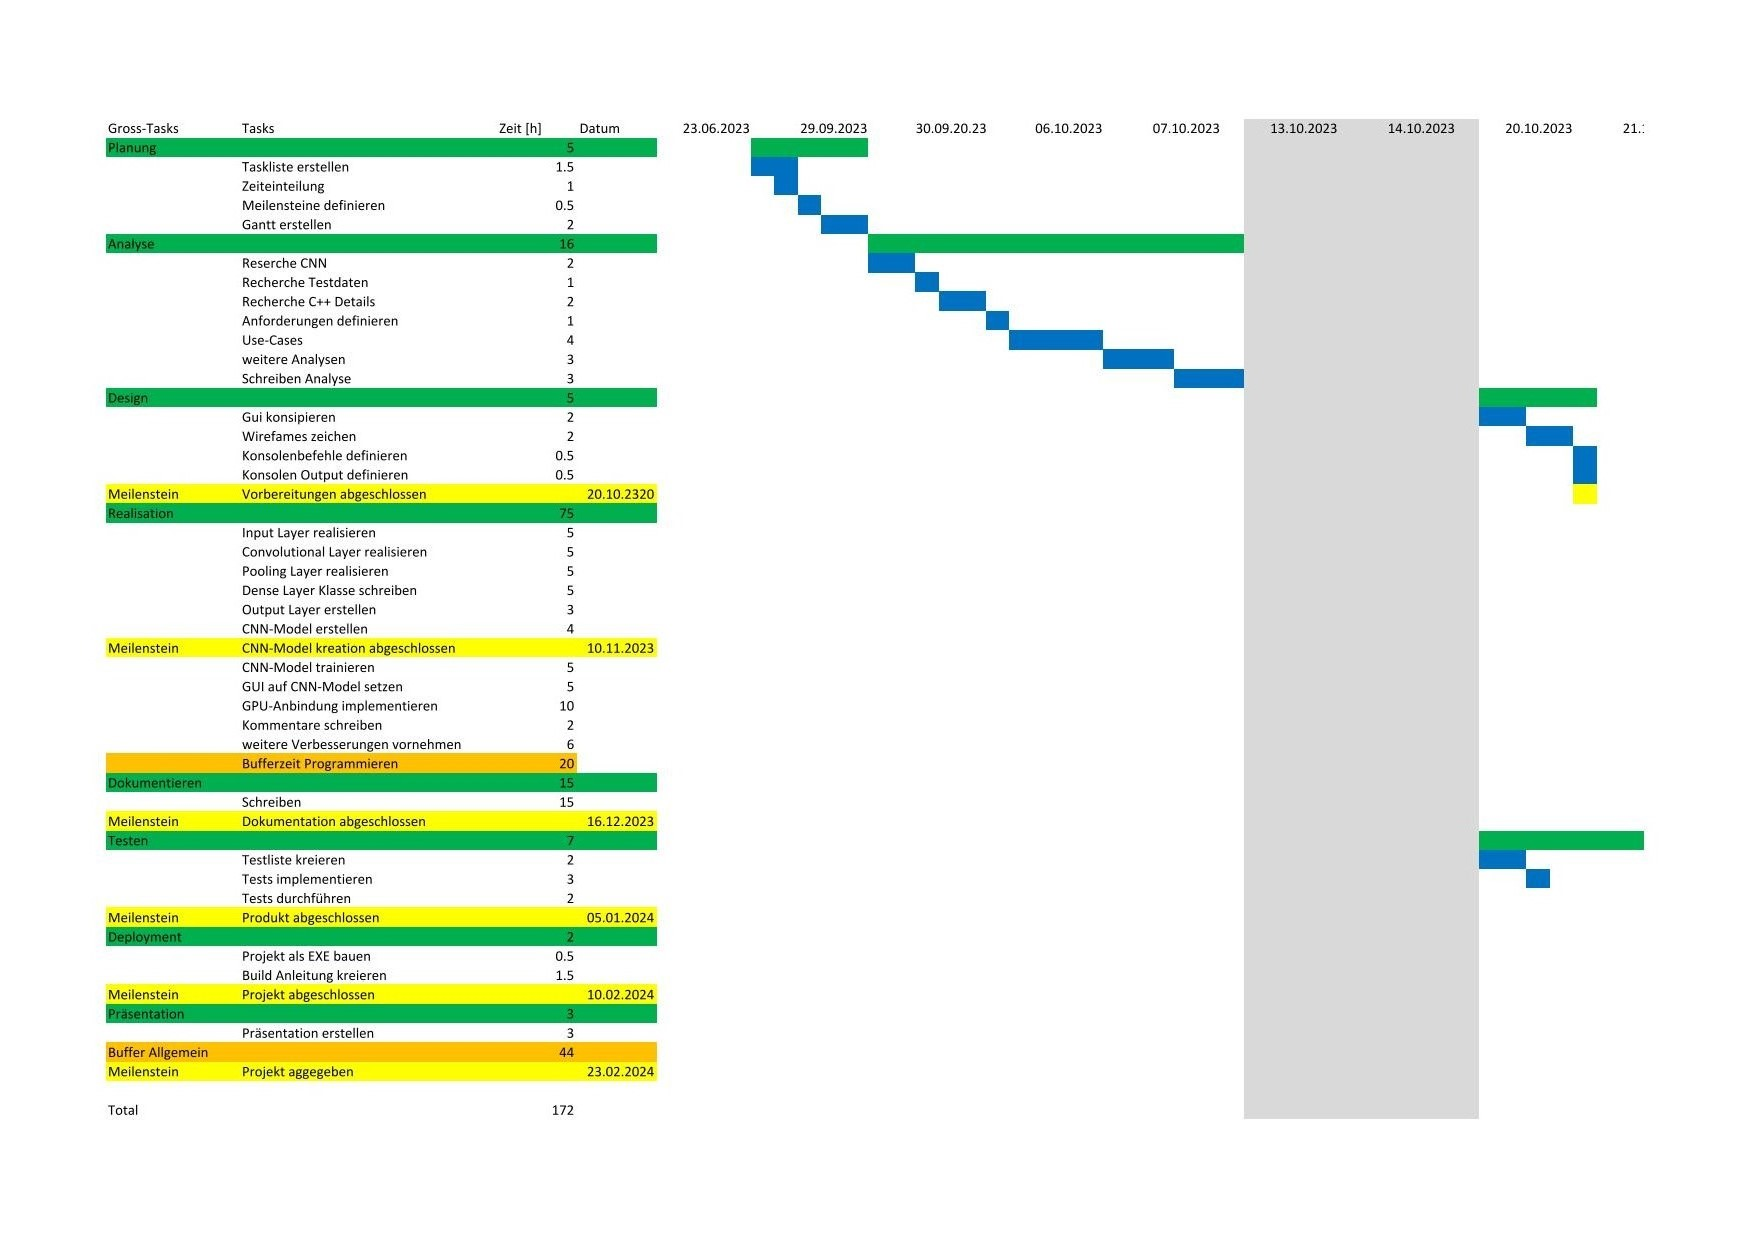
\includegraphics[width=\linewidth, height=\textheight, keepaspectratio]{gantt1_turned.jpg}
		\label{fig:gantt1}
	\end{figure}

	\begin{figure}[htbp]
		\centering
		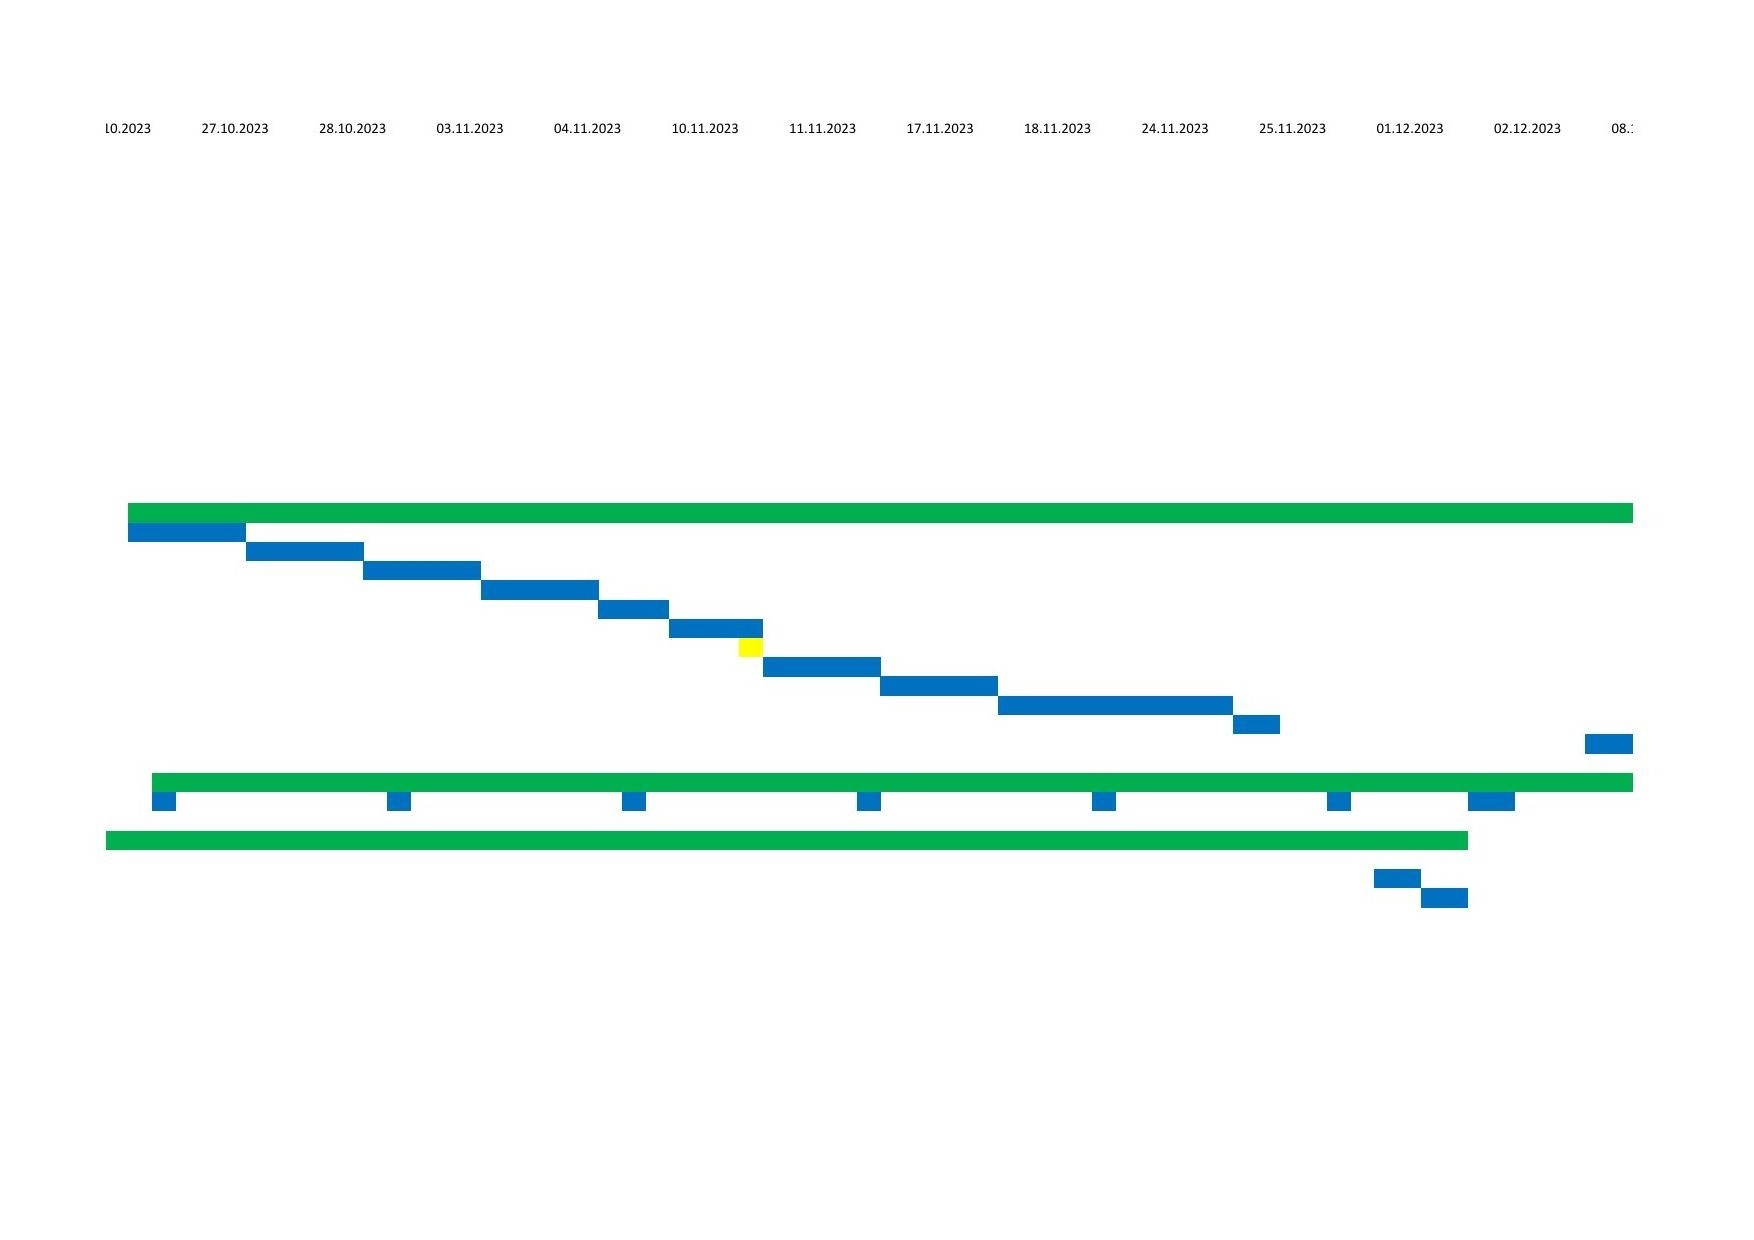
\includegraphics[width=\linewidth, height=\textheight, keepaspectratio]{gantt2_turned.jpg}
		\label{fig:gantt2}
	\end{figure}

	\begin{figure}[htbp]
		\centering
		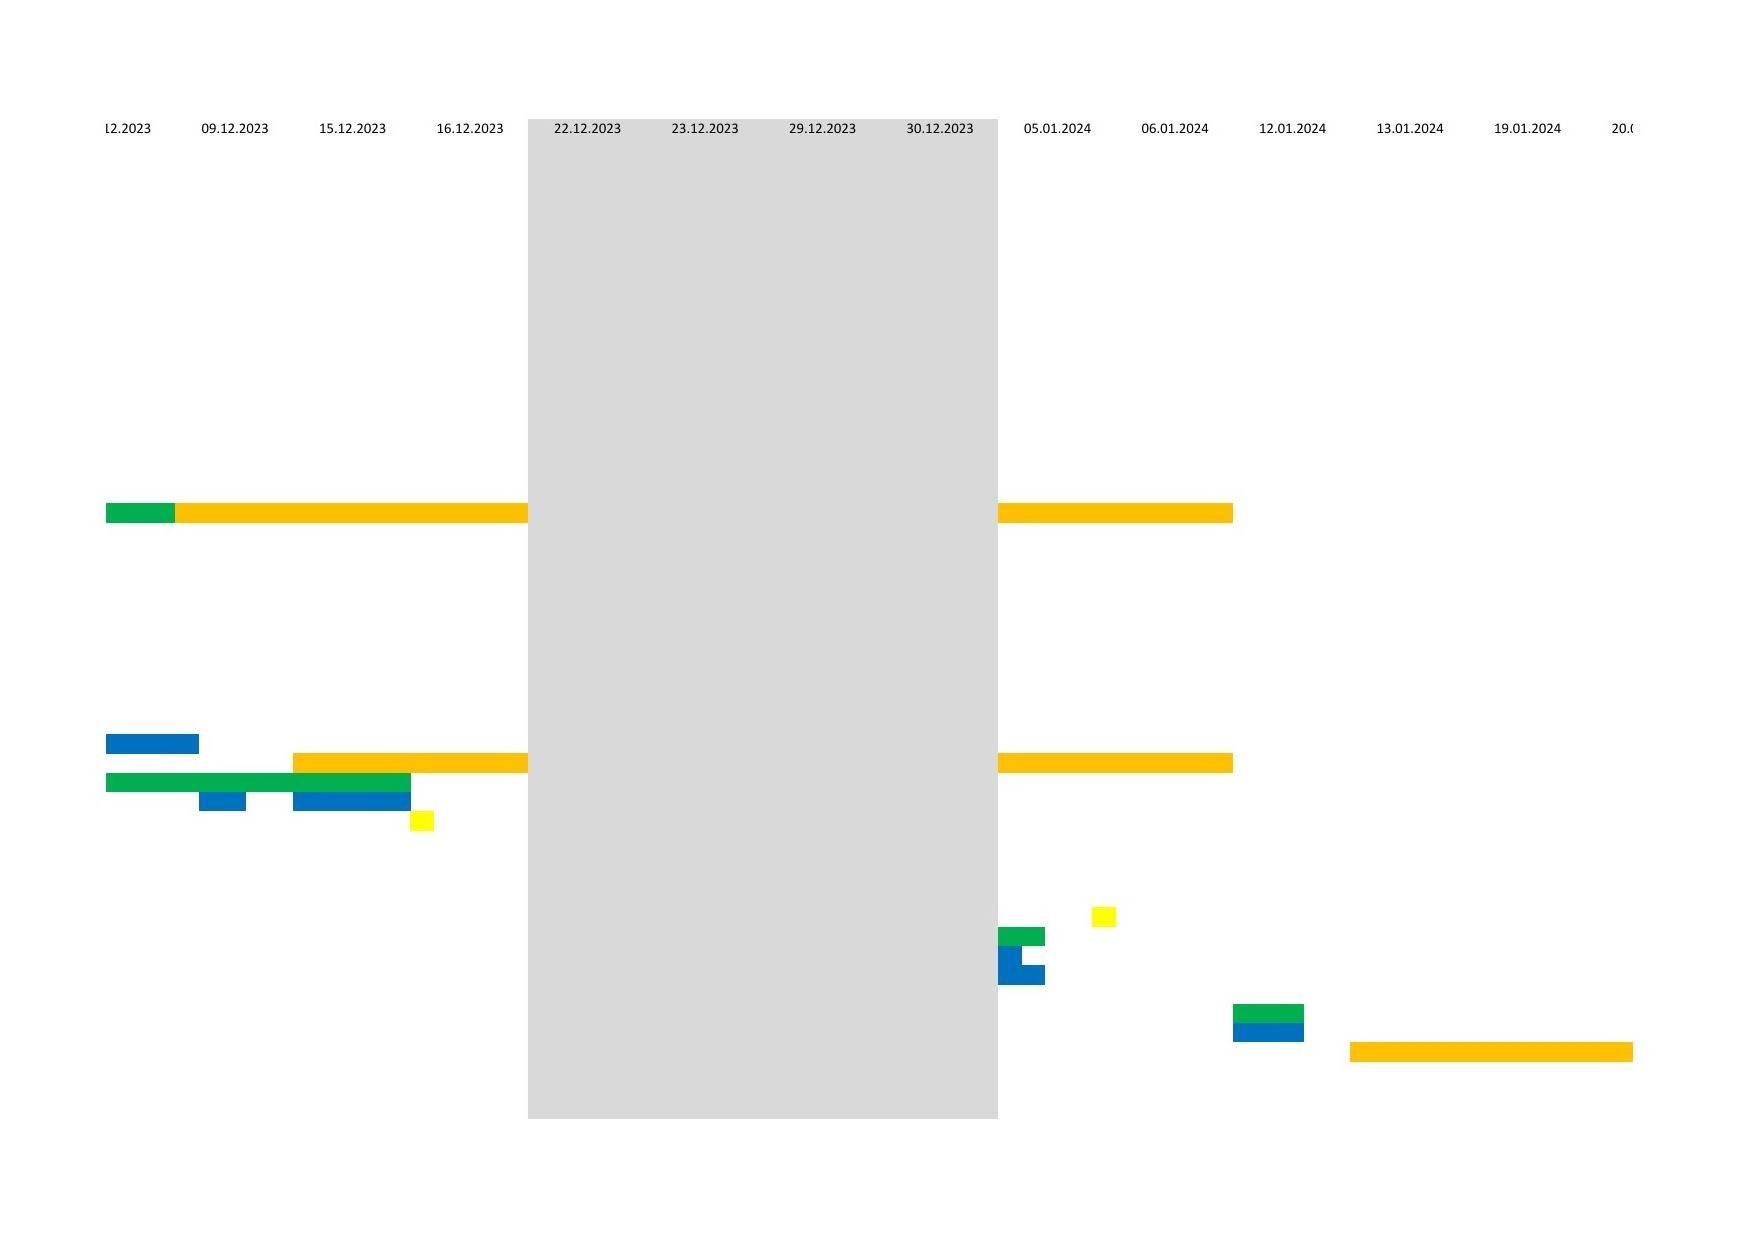
\includegraphics[width=\linewidth, height=\textheight, keepaspectratio]{gantt3_turned.jpg}
		\label{fig:gantt3}
	\end{figure}

	\begin{figure}[htbp]
		\centering
		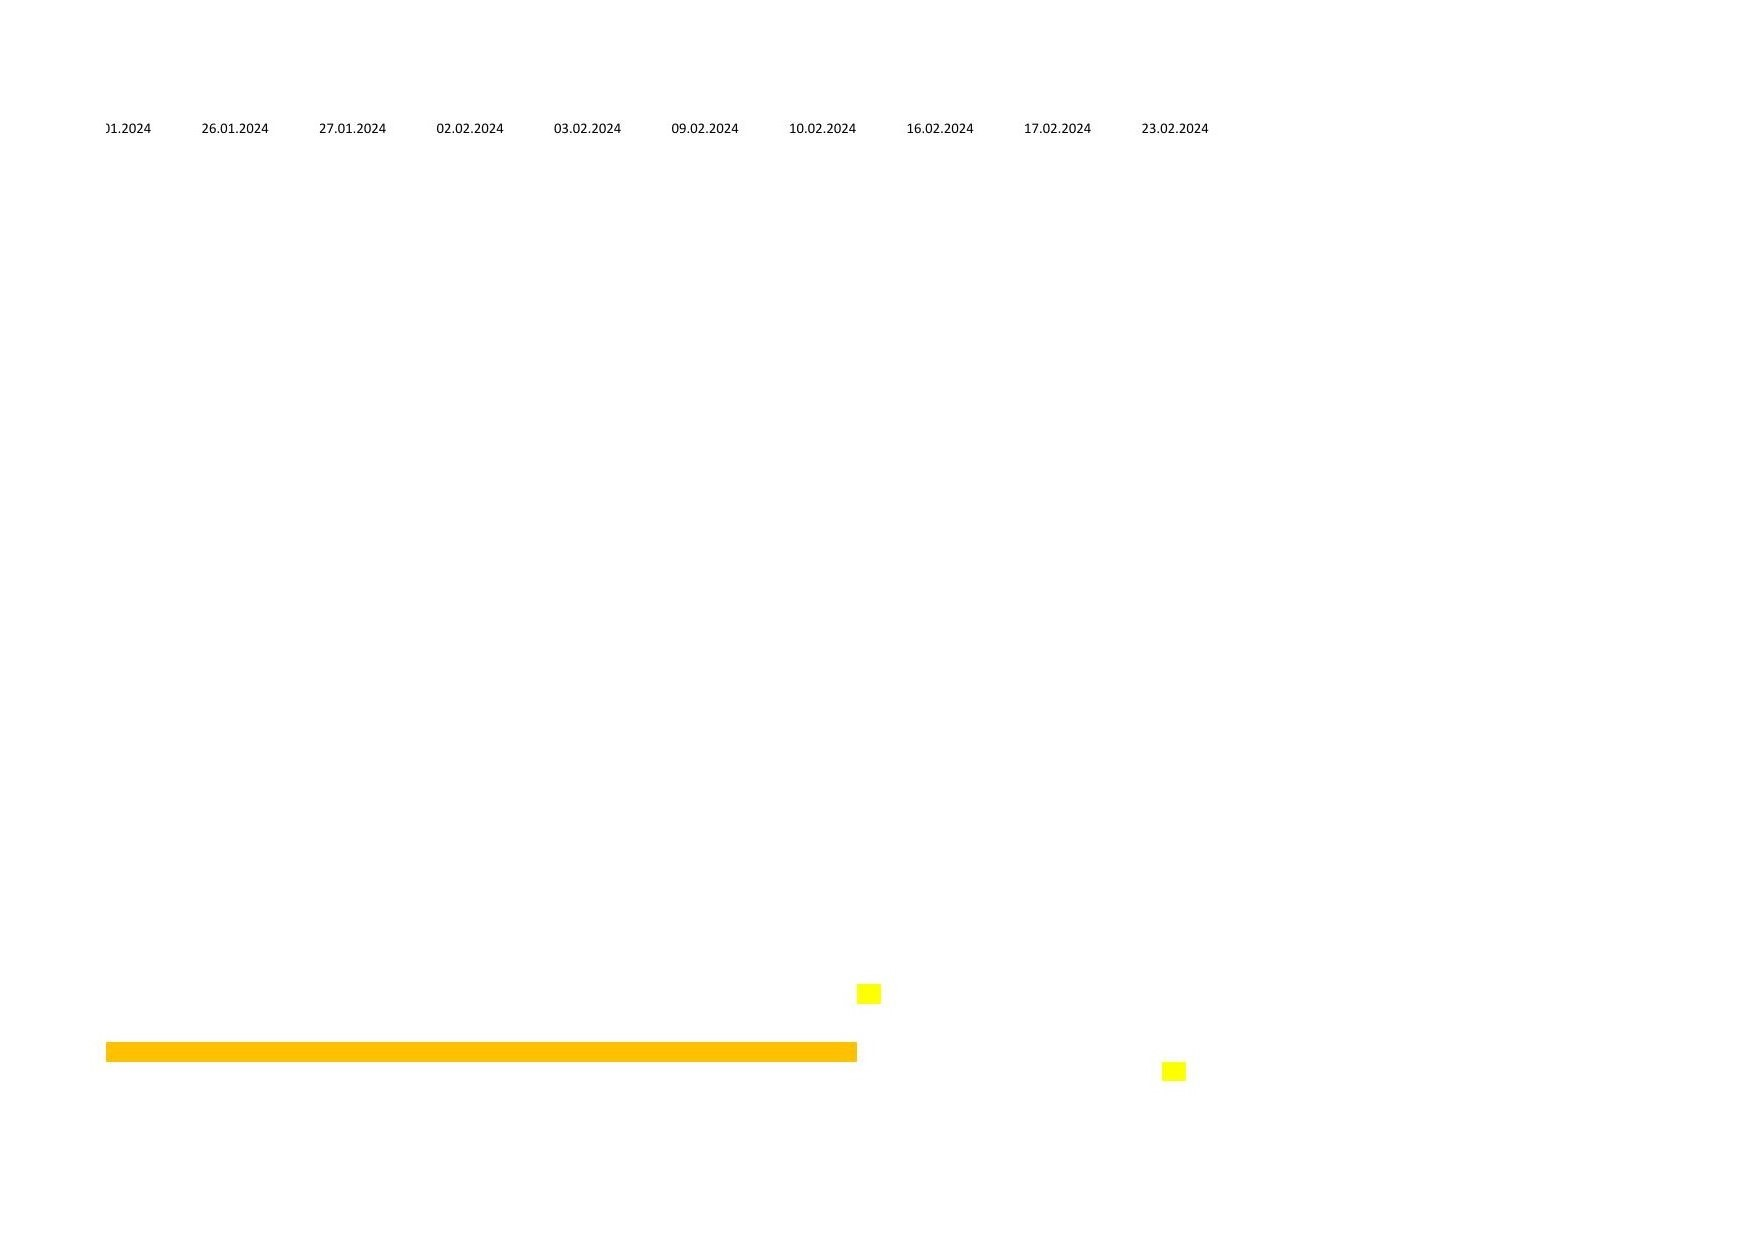
\includegraphics[width=\linewidth, height=\textheight, keepaspectratio]{gantt4_turned.jpg}
		\label{fig:gantt4}
	\end{figure}

\end{landscape}





%%Design
\chapter{Design}
\label{sec:Design}
\section{Konsole}
\label{sec:Konsole}
\subsection{Training}
\label{sec:Training}
\subsubsection{Input}
\label{sec:TraiInput}
\begin{lstlisting}[language=bash]
ki --training "[trainings.ubyte]"
\end{lstlisting}

\subsubsection{Output}
\label{sec:TraiOutput}
Nach jedem Datensatz wird angezeigt, wie viele der zum Training gegebenen Daten bereits abgearbeitet wurden. 

\subsection{Test}
\label{sec:Test}
\subsubsection{Input}
\label{sec:TestInput}
\begin{lstlisting}[language=bash]
ki --test "[test.ubyte]"
\end{lstlisting}

\subsubsection{Output}
\label{sec:TestOutput}
Nach jedem Datensatz wird angezeigt, wie viele der zum Testen gegebenen Daten bereits abgearbeitet wurden. Zudem wird angezeigt, wie viele der Datensatz richtig bzw. falsch erkannt wurden.



\subsection{Anwendung}
\label{sec:Anwendung}
\subsubsection{Input}
\label{sec:UseInput}
\begin{lstlisting}[language=bash]
ki "[image.jpg]"
\end{lstlisting}

\subsubsection{Output}
\label{sec:UseOutput}
Als Output werden alle Ziffern von 0 bis 9 mit den entsprechenden Prozentwerten zur�ckgegeben (Dies kommt daher, dass die KI die Wahrscheinlichkeit der �bereinstimmung f�r jede Ziffer berechnet.). Zudem wird auch angezeigt, welche Ziffer die h�chste �bereinstimmung hat. Da diese die erkannte Ziffer darstellt.

\section{Datenbank}
\label{sec:Datenbank}
Die Applikation ben�tigt keine Datenbank.

\section{Code}
\label{sec:Code}
\subsection{Klassendiagramm}
\label{sec:Klassendiagramm}
 Es gibt drei Klassen in CKi (Convolutional Layer, Pooling Layer, Dense Layers). Ein Convolutional Layer ist eine Art von Filter, welcher auf das Bild gelegt wird, um eine vereinfachte Erkennung zu erm�glichen. Die Pooling Layers sind verantwortlich das Bild zu verkleinern und so eine schnellere Verarbeitung zu erm�glichen. Die Dense Layers oder auch Fully Connected Layers sind das eigentlich das Gehirn der KI. Zus�tzlich gibt es die Main-Klasse, diese ist zust�ndig die oben genannten Klassen miteinander zu verbinden und so das Netzwerk aufzubauen. Zus�tzlich handhabt es die Nutzereingaben und die Auslese der Trainings-/Testdaten. 

\begin{figure}[H]
\centering
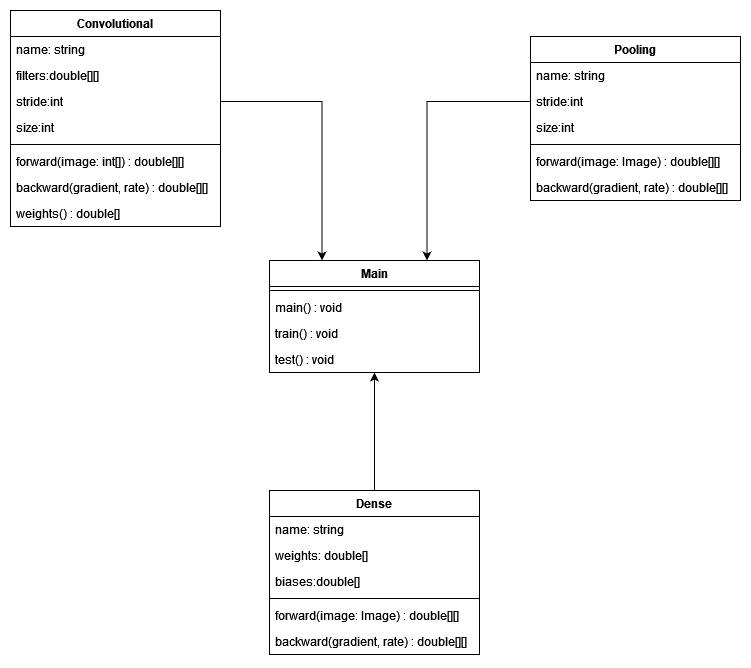
\includegraphics[height=0.5\paperheight]{Klassendiagramm.png}
\caption{Das Klassendiagramm, Grundaufbau der Applikation}
\label{fig:klassendiagramm}
\end{figure}

\subsection{Trainingsdaten}
\label{sec:Trainingsdaten}
Die Trainingsdaten sind das MNIST-Datenset mit den handschriftlichen Zahlen. (\url{http://yann.lecun.com/exdb/mnist/})

\subsection{Tests}
\label{sec:Tests}



%%Realisation
\chapter{Realisation}
\label{sec:Realisation}
\section{Allgemein}
\label{sec:RealAllgemein}
Die Realisation des Projekts CKI zeichnet sich durch die Implementierung eines modularen neuronalen Netzwerks aus, das für Aufgaben wie die Erkennung handschriftlicher Ziffern konzipiert wurde. Zum Einsatz kamen dabei Standard-C++-Technologien sowie eine CMake-basierte Projektstruktur für das Build-Management. Die Kernstruktur besteht aus Klassen für Neuron, Layer, und Network, die die Basis des Netzwerks bilden, ergänzt durch eine Util-Klasse für Hilfsfunktionen, wie Aktivierungsfunktionen und Datenverarbeitung.
Zusätzlich gibt es im Ordner „Test“ Unit-Tests mit den entsprechenden Attrappen für die MNIST-Datensätze. Die Unit-Tests sind mit Google-Tests implementiert.

\section{Abhängigkeiten}
\label{sec:RealAbhängigkeiten}
Das Projekt CKI kommt mit nur wenigen Abhängigkeiten aus.
Die, die es dennoch gibt, sind umso wichtiger für das erfolgreiche Ausführen der Applikation.
\\
Abhängigkeiten:
\begin{enumerate}
	\item \textbf{googletest:} \\
	\textbf{Version (Tag):} v1.14.0 \\
	\textbf{Git:} \url{https://github.com/google/googletest} \\
	\textbf{Beschreibung:} GoogleTest ist ein C++-Framework für Unit-Tests, das Assertions für die Überprüfung von Code und Funktionen für die Organisation und Ausführung von Tests bietet.

	\item \textbf{nlohmann/json:} \\
	\textbf{Version (Tag):} v3.11.3 \\
	\textbf{Git:} \url{https://github.com/nlohmann/json} \\
	\textbf{Beschreibung:} Nlohmann/json ist eine moderne, header-only C++ Bibliothek für die Verarbeitung von JSON-Daten, die einfache Integration und intuitive Nutzung bietet.

	\item \textbf{wichtounet/mnist:} (nicht mehr in Verwendung)\\
	\textbf{Version (Commit):} 3b65c35 \\
	\textbf{Git:} \url{https://github.com/wichtounet/mnist} \\
	\textbf{Beschreibung:} Wichtounet/mnist ist ein einfacher C++-Reader für den MNIST-Datensatz, der es ermöglicht, Trainings- und Testbilder sowie Labels zu lesen und zu verwenden.

	\item \textbf{nothings/stb:}\\
	\textbf{Version (Commit):} 5736b15 \\
	\textbf{Git:} \url{https://github.com/nothings/stb} \\
	\textbf{Beschreibung:} STB ist eine Sammlung plattformübergreifender Header-Dateien für C, die umfassende Funktionen für Grafik, Audio und Textverarbeitung ohne externe Abhängigkeiten bereitstellt. 
\end{enumerate}

\section{Architektur}
\label{sec:RealArchitektur}
\subsection{Klassen}
\label{sec:RealKlassen}
\subsubsection{Klassendiagramm}
\label{sec:RealKlassendiagramm}
\begin{figure}[H]
	\centering
		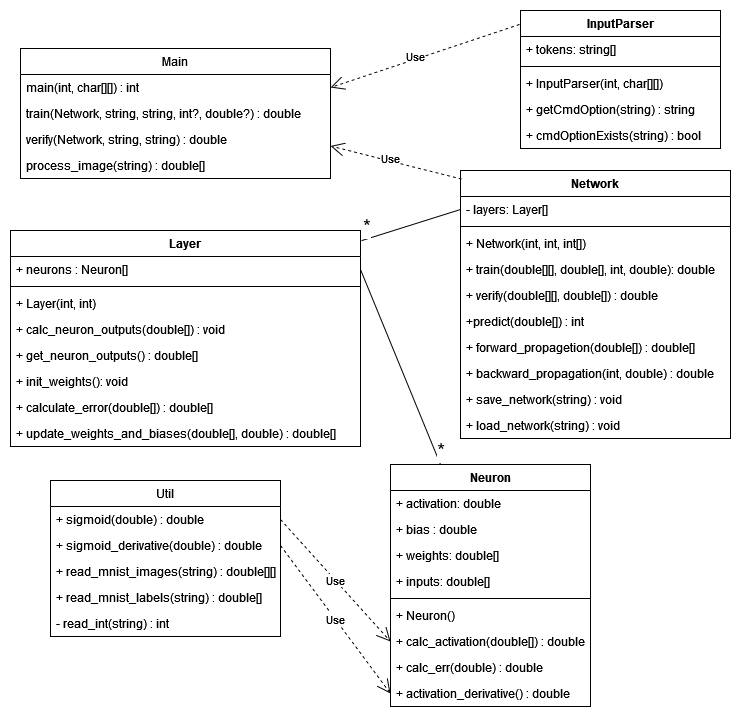
\includegraphics[width=1.00\textwidth]{klassendiagramm_after_implementation.png}
		\caption{Klassendiagramm nach der Realisation}
	\label{fig:klassendiagramm after implementation}
\end{figure}
Das ist das Klassendiagramm, wie die Applikation des Projektes CKI nach der Implementation aussieht. Somit sind die nötigen Anpassungen, die seit der Designphase zu treffen waren, ersichtlich.
\\
Wie zu sehen ist, gibt es etliche markante Änderungen in den Klassen Netzwerk und Layer. Dies kommt daher, dass in der Designphase aufgrund fehlendem oder unzureichendem Wissen die Struktur angepasst werden musste. Wie diese Klassen funktionieren, sowie die wichtigsten Funktionen sind in den Abschnitten \ref{sec:RealKlassen}, bis \ref{sec:RealSnippetsCode} zu finden. 
\\
Interessant ist die Klasse InputParser, welche beim ursprünglichen Entwurf nicht anzutreffen war. Diese Klasse ist zuständig, einzelne Attribute aus dem Aufruf der CKI-Main-Funktion auszulesen und eine einfache Verwendung dieser zu gewährleisten. Dabei ist diese Klasse nicht selbst implementiert, sondern stammt von \url{https://stackoverflow.com/questions/865668/parsing-command-line-arguments-in-c}. Dementsprechend wird im weiteren Verlauf nicht weiter auf diese Funktion eingegangen.

\subsubsection{Netzwerk}
\label{sec:RealNetzwerk}
Die Network-Klasse repräsentiert das neuronale Netzwerk. Es unterstützt die Initialisierung des Netzwerks mit einer bestimmten Anzahl von Eingabe- und Ausgabeneuronen sowie eine variable Anzahl von versteckten Schichten und deren Grössen. Die Klasse bietet Funktionen für das Training des Netzwerks mit gegebenen Eingaben und Zielwerten, die Überprüfung der Netzwerkleistung und Vorhersagen für neue Eingaben. Dies ist möglich wegen der Durchführung von Vorwärts- und Rückwärtspropagation, die wichtigsten Algorithmen im Bereich des maschinellen Lernens (Mehr dazu unter Algorithmen \ref{sec:RealAlgorithmen}).
\\
Zusätzlich existieren noch zwei Funktionen in der Klasse, welche zuständig sind für die Speicherung und das Laden des Netzwerks in bzw. aus einer Datei.

\subsubsection{Layer}
\label{sec:RealLayer}
Die Layer-Klasse definiert die Layer im neuronalen Netzwerk, bestehend aus mehreren Neuronen. Sie bietet Funktionen zum Initialisieren und Setzen von Gewichten, Berechnen der Ausgaben der Neuronen basierend auf Eingaben, Berechnen der Fehler im Vergleich zu den Zielwerten und der Aktualisierung von Gewichten und Biases auf Basis von Fehlern und Lernrate.Jedes Layer-Objekt enthält eine Liste von Neuron-Objekten, die die Neuronen in diesem Layer repräsentieren. 

\subsubsection{Neuron}
\label{sec:RealNeuron}
Die Neuron-Klasse stellt ein einzelnes Neuron dar, inklusive seiner Gewichte, 
Bias, Eingaben, Aktivierungsfunktion und Summe der gewichteten Eingaben. Sie bietet Funktionen zur Berechnung der Aktivierung basierend auf den Eingaben, der Ableitung der Aktivierungsfunktion, der Fehlerberechnung im Vergleich zu einem Zielwert, sowie zur Speicherung der Gewichte und des Biases.
\\
Zur Berechnung der Aktivierung und deren Ableitung werden die statischen Utility-Funktionen Sigmoid und die Ableitung von Sigmoid aus der Utility-Klasse genutzt (Siehe auch \ref{sec:RealSigmoidAbleitungCode}).

\subsubsection{Utility}
\label{sec:RealUtility}
Die Util-Klasse bietet statische Hilfsfunktionen für das neuronale Netzwerk, darunter die Sigmoid-Aktivierungsfunktion und ihre Ableitung sowie Funktionen zum Lesen von MNIST-Bilddaten und Labels aus Dateien. Diese Hilfsfunktionen sind essenziell für die Vorverarbeitung von Eingabedaten und die Implementierung der Lernmechanismen im Netzwerk. 

\subsection{Ordnerstruktur}
\label{sec:RealOrdnerstruktur}
Im Kern des Projekts stehen die Hauptdateien, welche die essenziellen Klassen wie Neuron, Layer, Network und Util enthalten. Diese sind grundlegend für die Funktionalität des neuronalen Netzwerks. Die CMakeLists.txt unterstützt das Build-Management, vereinfacht die Kompilierung und Konfiguration. Der .gitignore sorgt dafür, dass unnötige Dateien und Ordner nicht in die Versionskontrolle einfliessen. Ein speziell dafür vorgesehener Test-Ordner beinhaltet Tests zur Überprüfung der Funktionalität, was die Zuverlässigkeit des Systems sicherstellt. Zusätzlich runden Dummy-Files und ein eigener Ordner für die MNIST-Datasets das Projekt ab, indem sie das Vorhandensein der Datensets für Training und Tests des Netzwerks garantieren.
\\
Das CKI-Projekt ist strukturiert in:
\begin{itemize}
	\item \textbf{Hauptdateien:} (kein Ordner, Rootverzeichnis) 
	Enthalten die Klassen Neuron, Layer, Network, und Util für die Kernlogik des neuronalen Netzwerks.
  \item \textbf{CMakeLists.txt:} (Im Rootverzeichnis)
	Für das Build-Management erleichtert das Kompilieren und die Konfiguration des Projekts.
  \item \textbf{.gitignore:} (Im Rootverzeichnis)
	Definiert Dateien und Ordner, die von Git-Versionierung ausgeschlossen sind, wie Build-Artefakte und IDE-spezifische Dateien.
  \item \textbf{Test-Ordner:} 
	Beinhaltet Testfälle zur Überprüfung der Funktionalität einzelner Komponenten und des Gesamtsystems.
	
	\begin{itemize}
		\item \textbf{Dummy-Files:} 
		Zusätzliche Dateien für Testzwecke. 
		\item \textbf{Unittests:}
		Tests zur Sicherstellung korrekter Funktionalität, Isolation von Fehlern. 
	\end{itemize}
	\item \textbf{MNIST-Datasets Ordner:} 
	Speichert die Datensätze für das Training und Testen des Netzwerks, insbesondere für die Erkennung handschriftlicher Ziffern.
\end{itemize}

\section{Code}
\label{sec:RealCode}
\subsection{Konzept}
Das Projekt CKI nutzt grundlegende Konzepte des maschinellen Lernens wie Vorwärts- und Rückwärts-Propagierung, Aktivierungsfunktionen (hier Sigmoid) und die Anpassung von Gewichten während des Trainingsprozesses. Die modulare Struktur, unterteilt in Schichten, Neuronen und Hilfsfunktionen, sowie die reine objektorientierte Implementation in C++ ohne externe Bibliotheken, abgesehen von Bibliotheken für Tests und Datenhandling, zeichnen die Architektur der Applikation aus.
\\
Um mehr über die hier erwähnten Funktionen zu erfahren, ist der Abschnitt \ref{sec:RealAlgorithmen} zu konsultieren.

\subsection{Algorithmen}
\label{sec:RealAlgorithmen}
\subsubsection{ Forward-Propagation}
\label{sec:RealForwardPropagation}
Die Forward-Propagation ist ein grundlegender Prozess in neuronalen Netzwerken, der es ermöglicht, Vorhersagen auf Basis von Eingabedaten zu treffen. Dabei werden die Eingabedaten durch das Netzwerk von der Eingabeschicht über eine oder mehrere versteckte Schichten bis zur Ausgabeschicht vorwärts geleitet. Jede Schicht besteht aus Neuronen, die über Gewichte mit den Neuronen der vorherigen Schicht verbunden sind. Die Daten werden in jedem Neuron durch eine Summationsfunktion verarbeitet, die die gewichteten Eingaben aufsummiert und einen Bias-Wert hinzufügt. Das Ergebnis dieser Summation wird dann durch eine Aktivierungsfunktion geleitet, um die Ausgabe des Neurons zu bestimmen.
\\
Die Aktivierungsfunktion bestimmt, wie Neuronen ihre Eingaben in Ausgaben umwandeln und ist entscheidend für die Fähigkeit des Netzwerks, komplexe Muster in den Daten zu erkennen. Beliebte Aktivierungsfunktionen sind die Sigmoid-, Tanh- und ReLU-Funktion.\footnote{vgl. Li \& Johnson \& Yeung, 2017; databasecamp, 2023}
\\
Sobald die Eingabedaten durch das Netzwerk propagiert worden sind und die Ausgabeschicht erreicht haben, wird das Ergebnis mit dem tatsächlichen Wert verglichen, um den Fehler der Vorhersage zu bestimmen. Dieser Fehler wird dann in einem separaten Prozess, der als Backpropagation bekannt ist, verwendet, um die Gewichte im Netzwerk anzupassen und die Vorhersagegenauigkeit zu verbessern.\footnote{vgl. Nüesch, 2023;  3Blue1Brown, 2017;}
%TODO add Math
\subsubsection{Back-Propagation}
\label{sec:RealBackPropagation}
Die Backpropagation, kurz für „backward propagation of errors“, ist ein Schlüsselmechanismus im Training neuronaler Netzwerke. Dieser Algorithmus ermöglicht es, die Gewichte des Netzwerks so anzupassen, dass der Gesamtfehler bei der Vorhersage minimiert wird. Backpropagation wird nach der Forward-Propagation angewendet, nachdem eine Vorhersage durch das Netzwerk gemacht und der Fehler zwischen der Vorhersage und dem tatsächlichen Wert berechnet wurde.
\\
Der Prozess der Backpropagation besteht aus zwei Hauptphasen: der Berechnung des Gradienten des Fehlers bezüglich aller Gewichte im Netzwerk und der anschliessenden Anpassung dieser Gewichte in die Richtung, die den Fehler minimiert. Der Gradient gibt an, in welche Richtung die Gewichte verändert werden müssen, um den Fehler zu verringern, und die Grösse der Anpassung wird durch die Lernrate bestimmt.
\\
Backpropagation nutzt die Kettenregel der Differenzialrechnung, um die Fehlergradienten für die Gewichte jeder Schicht vom Ausgang zurück zum Eingang effizient zu berechnen. Der berechnete Fehlergradient für jede Gewichtung zeigt, wie eine kleine Änderung in diesem Gewicht den Gesamtfehler beeinflusst. Durch die systematische Anpassung der Gewichte basierend auf diesen Gradienten kann das Netzwerk schrittweise verbessert werden, um genauere Vorhersagen zu liefern.
\\
Insgesamt ermöglicht Backpropagation das effiziente Training tiefer neuronaler Netzwerke, indem es systematisch die Netzwerkgewichte anpasst, um den Fehler zwischen den Vorhersagen des Netzwerks und den tatsächlichen Werten zu minimieren, was zu einer verbesserten Modellleistung führt.\footnote{vgl. Nüesch, 2023; 3Blue1Brown, 2017; Karpathy, 2016; Roy, 2022; Li \& Johnson \& Yeung, 2017; }
%TODO add Math
\subsection{Schlüsselpassagen \& Snippets}
\label{sec:RealSnippetsCode}
Die wichtigsten Funktionen in einem neuronalen Netzwerk sind die beiden Propagation, vorwärts als auch rückwärts. Wobei diese das Grundgerüst für die drei Hauptfunktionen, Train, Verify \& Predict bilden.

\subsubsection{Train}
\label{sec:RealTrainCode}
\begin{lstlisting}[language=C++]
double Network::train(std::vector<std::vector<double>> &inputs, std::vector<double> &labels, int epochs, double learning_rate){
    double total_error = 0;
    for(int epoch = 0; epoch<epochs; epoch++ ){
        for(std::size_t i = 0; i < inputs.size(); i++){
            std::vector<double> outputs = Network::forward_propagation(inputs[i]);
            total_error += Network::backward_propagation(labels[i], learning_rate);
            total_error /= 2;
        }
    }
    return total_error;
}

\end{lstlisting}
\addcontentsline{lol}{lstlisting}{\protect\numberline{\thelstlisting} Train Funktion aus der Netzwerk-Klasse}
Die Funktion, welche für das Lernen des neuronalen Netzwerks verantwortlich ist, ist simpel aufgebaut. Sie erhält primär zwei Listen: eine Liste aus Bildern und eine Liste aus Beschriftungen für die Bilder. Danach nutzt Train die Funktionen der Forward- und Back-Propagation, um zuerst das Bild durch das Netzwerk bewerten zulassen und dann diese Bewertung mithilfe der Beschriftungen zu korrigieren. Dies tut sie für den gesamten Datensatz oder durch eine zukünftige Erweiterung in einzelnen Blöcken (für höhere Effektivität) und der Anzahl Epochen entsprechend.

\subsubsection{Verify}
\label{sec:RealVerifyCode}
\begin{lstlisting}[language=C++]
double Network::verify(const std::vector<std::vector<double>> &inputs, const std::vector<double> &labels){
    int correct = 0;
    for (std::size_t i = 0; i < inputs.size(); ++i){
        if (Network::predict(std::vector<double>(inputs[i])) == static_cast<int>(labels[i])){
            correct++;
        }
    }
    return static_cast<double>(correct) / static_cast<double>(inputs.size());
}
\end{lstlisting}
\addcontentsline{lol}{lstlisting}{\protect\numberline{\thelstlisting} Verify Funktion aus der Netzwerk-Klasse}
Die Funktion ist eigentlich gleich aufgebaut wie „Train“, jedoch mit dem markanten Unterschied, dass keine Back-Propagation zum Einsatz kommt. So werden die Bewertungen des neuronalen Netzwerks nur als richtig oder falsch bewertet und nicht korrigiert.

\subsubsection{Predict}
\label{sec:RealPredictCode} %TODO change code...
\begin{lstlisting}[language=C++]
int Network::predict(const std::vector<double> &input){
    std::vector<double> outputs = Network::forward_propagation(input);
    return static_cast<int>(std::distance(outputs.begin(), std::max_element(outputs.begin(), outputs.end())));
}
\end{lstlisting}
\addcontentsline{lol}{lstlisting}{\protect\numberline{\thelstlisting} Predict Funktion aus der Netzwerk-Klasse}
Diese Funktion erhält nur ein einziges Bild als Attribut. Dieses Bild wird durch die Forward-Propagation bewertet. Die Bewertung wiederum besteht nur aus einer Liste von zehn Prozentzahlen (für die Ziffern von 0 bis 9) und damit diese besser für einen Menschen lesbar wird, muss die höchste Prozentzahl aus der Liste gesucht werden. Deren Index wird dann als errechnete Zahl zurückgegeben.
\\
(Diese Funktion ist ein Zusammenzug aus der Predic-Funktion und Logic aus der main.cpp-Datei.) %FIXME if code changes remove

\subsubsection{Forward-Propagation}
\label{sec:RealForwardPropagationCode}
\begin{lstlisting}[language=C++]
std::vector<double> Network::forward_propagation(const std::vector<double>& input){
    layers[0].calc_neuron_outputs(input);

    for (int i = 1; i < layers.size(); ++i){
        std::vector<double> inputs = layers[i - 1].get_neuron_outputs();
        layers[i].calc_neuron_outputs(inputs);
    }

    return layers[layers.size()-1].get_neuron_outputs();
}
\end{lstlisting}
\addcontentsline{lol}{lstlisting}{\protect\numberline{\thelstlisting} Forward-Propagation Funktion aus der Netzwerk-Klasse}
In dieser Funktion wird eine Liste von grossen Fliesskommazahlen übernommen. Diese sind die einzelnen Pixel, in dem zu bearbeiteten Bild, welche nur einen Helligkeitswert beinhalten. Diese Pixel werden an den ersten Layer im Netzwerk übergeben. Dieser kalkuliert durch die Sigmoid-Funktion neue Ausgabewerte. Die Ausgabewerte werden mit der For-Schleife durch alle Schichten des Netzwerks weitergereicht, bis diese am Ende ausgelesen und als Rückgabewert dieser Funktion genutzt werden. Die Ausgabewerte haben zwar das gleiche Datenformat, unterscheiden sich jedoch anhand ihrer Grösse (Länge der Liste) und den tatsächlichen Werten.

\subsubsection{Back-Propagation}
\label{sec:RealBackPropagationCode}
\begin{lstlisting}[language=C++]
double Network::backward_propagation(const int& target, double learning_rate){
    std::vector<double> inputs (10, 0);
    inputs[target] = 1;
    std::vector<double> error = layers[layers.size()-1].calculate_error(inputs);

    double total_error = 0;
    for(double& e : error) { //remove for better performance
        total_error += e;
    }

    total_error/=error.size();

    //std::cout << total_error << std::endl;

    for (int i = layers.size() - 1; i >= 0; --i){
        error = layers[i].update_weights_and_biases(error, learning_rate);
    }
    return total_error;
}
\end{lstlisting}
\addcontentsline{lol}{lstlisting}{\protect\numberline{\thelstlisting} Backward-Propagation Funktion aus der Netzwerk-Klasse}
Im Gegensatz zur Forward-Propagation wird in der Back-Propagation ein Wert nicht von der ersten Schicht zur letzten übergeben, sondern Rückwerts von dem letzten Layer bis zur Eingabe zurück.
\\ 
Dabei muss zuerst die Abweichung von der erhaltenen Ausgabe (aus der Forward-Propagation) mit der erwarteten Ausgabe abgeglichen und der Fehler berechnet werden. Nun wird ähnlich zur Forward-Propagation dieser Fehler durch die einzelnen Schichten geschickt und dort verwendet, um die Gewichtungen und Biases für jedes Neuron anzupassen. Dies passiert in einer eigenen Funktion im Layer.

\subsubsection{Anpassung von Gewichtungen und Biases}
\label{sec:RealAnpassungVonGewichtungenUndBiasesCode}
\begin{lstlisting}[language=C++]
std::vector<double> Layer::update_weights_and_biases(const std::vector<double>& error, double learning_rate){
    std::vector<double> prev_layer_error(Layer::neurons[0].weights.size(), 0.0);

    for (size_t i = 0; i < Layer::neurons.size(); ++i){
        Neuron &neuron = Layer::neurons[i];
        const double neuron_error = error[i];
        const double activation_derivative = neuron.activation_derivative();

        for (size_t j = 0; j < neuron.weights.size(); ++j){
            prev_layer_error[j] += neuron.weights[j] * neuron_error;

            const double delta_weight = neuron_error * activation_derivative * neuron.inputs[j];
            neuron.weights[j] -= learning_rate * delta_weight;
        }
        neuron.bias += learning_rate * neuron_error * activation_derivative;
    }
    return prev_layer_error;
}
\end{lstlisting}
\addcontentsline{lol}{lstlisting}{\protect\numberline{\thelstlisting} Anpassung von Gewichtungen und Biases aus der Layer-Klasse}
Dies ist die Funktion, die in der Back-Propagation aufgerufen wird.
\\
Dabei wird für jedes Neuron für jede Gewichtung eine eigene Anpassung gesucht. Um dies zu erreichen, werden mehrere Werte benötigt: 
Der Fehler des Neurons, der Input des Neurons, die Ableitung der Aktivierung und die Learningrate.
Nun können die Änderungen bei der Gewichtung und dem Bias berechnet werden. Die Abweichung der Gewichtung ist ein Produkt des Inputs in diesem Neuron, dem Fehler, der Ableitung der Sigmoid-Funktion und der Learningrate. Die Korrektion für das Bias ist fast identisch zur Abweichung der Gewichtung. Es ist ebenfalls ein Produkt der gleichen Faktoren, abgesehen von der Learningrate und dem Input.
\\
Zusätzlich kann der Fehler für den nächsten Layer berechnet werden. Dieser wird benötigt, um die Backpropagation auf den nächsten Layer auszudehnen und dort dieselben Schritte auszuführen. Dabei setzt sich der Fehler für den nächst oberen Layer auseinander, aus dem
Fehler und dem entsprechenden Gewicht für das Neuron. Dabei wird der 
Fehler neu gewichtet und zusammen mit allen anderen neu-gewichteten Fehlern für dieses eine Neuron auf der nächsten Ebene aufsummiert.

\subsubsection{Sigmoid \& Ableitung}
\label{sec:RealSigmoidAbleitungCode}
\begin{lstlisting}[language=C++]
double Util::sigmoid(double x){
	return 1.0 / (1.0 + exp(-x));
}

double Util::sigmoid_derivative(double x){
	double s = sigmoid(x);
	return s * (1.0 - s);
}
\end{lstlisting}
\addcontentsline{lol}{lstlisting}{\protect\numberline{\thelstlisting} Sigmoid \& Ableitung aus der Util-Klasse}
Das sind die mathematischen Implementierungen der Sigmoid-Funktion und deren mathematischen Abweichungen. Diese Funktionen sind zuständig für die einzelnen Aktivierungen der Neuronen und verschieben eine Zahl in den Wertebereich zwischen 0 und 1.
\begin{figure}[H]
	\centering
		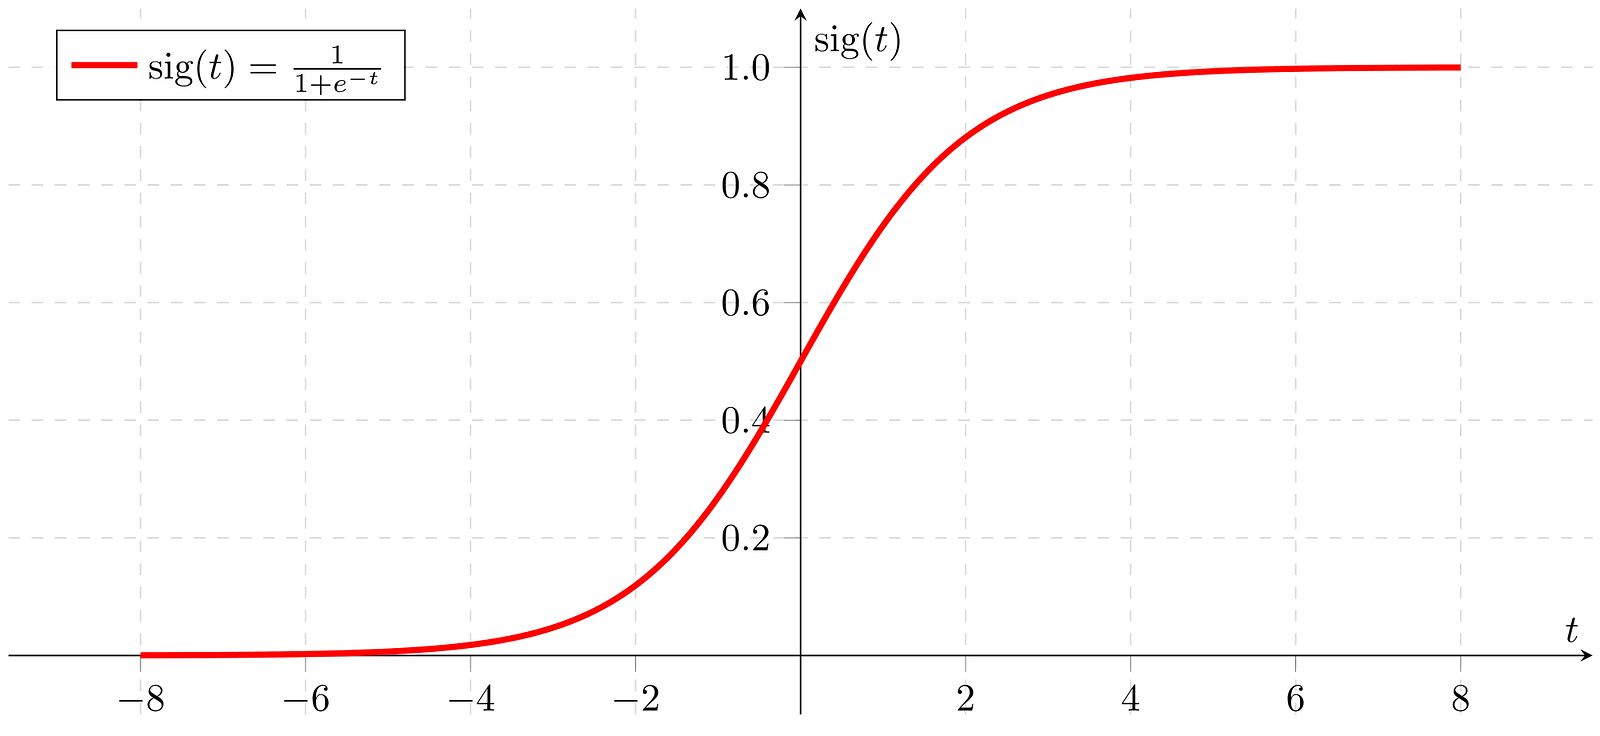
\includegraphics[width=0.75\linewidth]{sigmoid.png}
		\caption{Sigmoid Funktion}
	\label{fig:sigmoid}
\end{figure}

\subsubsection{MNIST-Reader}
\label{sec:RealMNISTReaderCode}
\begin{lstlisting}[language=C++]
std::vector<std::vector<double>> Util::read_mnist_images(const std::string &filename){
    std::ifstream file(filename, std::ios::binary);
    if (file.is_open()){
        int magic_number = read_int(file);
        int number_of_images = read_int(file);
        int number_of_rows = read_int(file);
        int number_of_columns = read_int(file);

        std::vector<std::vector<double>> images(number_of_images, std::vector<double>(number_of_rows * number_of_columns));

        for (int i = 0; i < number_of_images; ++i){
            for (int r = 0; r < number_of_rows * number_of_columns; ++r){
                unsigned char temp = 0;
                file.read(reinterpret_cast<char*>(&temp), sizeof(temp));
                images[i][r] = (double)temp / 255.0; // Normalizing pixel values to [0, 1]
            }
        }
        return images;
    }else{
        throw std::runtime_error("Cannot open file: " + filename);
    }
}
\end{lstlisting}
\addcontentsline{lol}{lstlisting}{\protect\numberline{\thelstlisting} MNIST-Reader aus der Util-Klasse}
Um die Daten aus den von \url{http://yann.lecun.com/exdb/mnist/} stammenden UByte-Dateien auszulesen, müssen gewisse Byte-Werte aus den Dateien ausgelesen werden. Die hier aufgeführte Funktion dient dazu, Bilder aus diesen Dateien auszulesen und ist beispielhaft auch für die Labels.
\\
Die Implementierung ist nach dem Muster von \url{http://yann.lecun.com/exdb/mnist/} implementiert. So sind in den ersten vier Byte gespeichert, wie viele Bilder/Beschriftungen im Datensatz zu finden sind. Um dies auszulesen, ist in einer eigenen Funktion implementiert (read\_int). Nach den ersten vier Byte müssen die restlichen Bytes in eine Liste eingetragen, in eine ganze Zahl interpretiert (zwischen 0 und 255) und auf den Wert zwischen 0 und 1 gebracht werden. Man spricht auch von der Normalisierung der Pixel-Werte.

\subsubsection{Ersten 4 Bytes}
\label{sec:RealErsten4BytesCode}
Dies ist die oben angesprochene „read\_int“-Funktion.
\begin{lstlisting}[language=C++]
int Util::read_int(std::ifstream &file){
    unsigned char bytes[4];
    file.read(reinterpret_cast<char*>(bytes), sizeof(bytes));
    return (int)((bytes[0] << 24) | (bytes[1] << 16) | (bytes[2] << 8) | bytes[3]);
}
\end{lstlisting}
\addcontentsline{lol}{lstlisting}{\protect\numberline{\thelstlisting} Utility Funktion für den MNIST-Reader aus der Util-Klasse}
Die Funktion wurde mit der Hilfe von Stack Overflow unter dem Link \url{https://stackoverflow.com/questions/604431/c-reading-unsigned-char-from-file-stream} erstellt.
\\
Zuerst wird ein Array in der Grösse von vier Bytes erstellt und vier Bytes aus einer Datei eingelesen. Danach werden die vier Bytes zu einer einzigen ganzen Zahl zusammengesetzt. Dies geschieht, indem die Bytes um jeweils 8 Bits nach Links verschoben werden und somit das erste Byte die acht höchsten Stellen der ganzen Zahl symbolisiert, danach das zweite Byte und so folgend die restlichen Bytes.

\subsubsection{Bild Vorverarbeitung}
\label{sec:RealBildVorverarbeitungCode}
\begin{lstlisting}[language=C++]
std::vector<double> process_image(const char* filename) {
    int width, height, channels;
    unsigned char* img = stbi_load(filename, &width, &height, &channels, 0);
    if (img == nullptr) {
        std::cerr << "Error in loading the image" << std::endl;
        exit(1);
    }

    unsigned char* resized_img = new unsigned char[28 * 28 * channels];
    stbir_resize_uint8(img, width, height, 0, resized_img, 28, 28, 0, channels);

    std::vector<double> image_data(28 * 28);
    for (int i = 0; i < 28 * 28; ++i) {
        int j = i * channels;
        double gray = 0.299 * resized_img[j] + 0.587 * resized_img[j + 1] + 0.114 * resized_img[j + 2];
        image_data[i] = gray / 255.0; // Normalize to [0, 1]
    }

    stbi_image_free(img);
    delete[] resized_img;

    return image_data;
}
\end{lstlisting}
Dies Funktion lädt ein Bild von der angegebenen Datei, skaliert es auf 28x28 Pixel herunter und konvertiert es in Graustufen. Zuerst wird das Bild geladen, wobei Breite, Höhe und Kanäle des Bildes erfasst werden. Falls das Laden fehlschlägt, wird eine Fehlermeldung ausgegeben und das Programm beendet. Anschließend wird das Bild auf die Größe 28x28 Pixel verkleinert, wobei die Anzahl der Kanäle beibehalten wird. Danach wird für jeden Pixel ein Graustufenwert berechnet, indem eine gewichtete Summe seiner RGB-Werte gebildet und durch 255 geteilt wird, um den Wert auf den Bereich [0, 1] zu normalisieren. Diese Werte werden gespeichert und am Ende der Funktion zurückgegeben. Zum Schluss werden der Speicher des ursprünglichen und des skalierten Bildes freigegeben, um Speicherlecks zu verhindern.
\\
Diese Funktion wird verwendet, um in der Ausführung von Predict das Bild des Nutzers zu übernehmen und auf das geforderte Format zu verkleinern.

%%Testing
\chapter{Testing}
\label{sec:Testing}
\section{Unittests}
\label{sec:DesignUnitTesting}
Beim Unit-Testing wird Code durch Code überprüft. So kann die Integrität des Projektes von einer einzelnen Funktion zu ganzen Klassen vom Grund auf überprüft werden.
\\
In CKI werden die Klassen für das Neuron, den Layer und das Netzwerk getestet. Zusätzlich gibt es Tests zu den meisten Funktionen der Utility-Klasse.
\\
Dabei werden Unit-Tests in CKI mit der „Google-Tests“ Bibliothek von Google implementiert.

\subsection{Util (Utility-Klasse)}
\label{sec:DesignUtilUtilityKlasse}
\subsubsection{Sigmoid-Funktionstests}
\label{sec:DesignSigmoidFunktionstests}
Prüfen, ob die Sigmoid- und ihre Ableitungsfunktion die erwarteten Werte zurückgeben.
\subsubsection{Dateilese-Tests}
\label{sec:DesignDateileseTests}
Überprüfen das korrekte Lesen eines Integers aus einer Binärdatei und das korrekte Verhalten beim Versuch, nicht vorhandene Dateien zu lesen.
\subsubsection{MNIST-Daten-Tests}
\label{sec:DesignMNISTDatenTests}
Überprüfen das Einlesen von MNIST-Bild- und Label-Daten, einschliesslich der Überprüfung der Anzahl und der Normalisierung von Bildern sowie der Überprüfung der Gültigkeit von Labels.

\subsection{Network}
\label{sec:DesignNetwork}
\subsubsection{Index in akzeptiertem Bereich}
\label{sec:DesignIndexInAkzeptiertemBereich}
Überprüft, ob die predict-Methode einen gültigen Index innerhalb des erwarteten Bereichs zurückgibt.
\subsubsection{Training beeinflusst das Verhalten.}
\label{sec:DesignTrainingBeeinflusstDasVerhalten}
Testet, ob das Training des Netzwerks dessen Verhalten ändert, indem es die Ausgaben vor und nach dem Training vergleicht. Es wird festgestellt, dass sich die Ausgaben verändern sollten, was auf eine Modifikation des Netzwerks hinweist.
\subsubsection{Netzwerkspeicher}
\label{sec:DesignNetzwerkspeicher}
Überprüft die Funktionalität zum Speichern und Laden des Netzwerks. Nach dem Speichern und Laden wird erwartet, dass das Netzwerk wie vorgesehen funktioniert.

\subsection{Layer}
\label{sec:DesignLayer}
\subsubsection{Initialisierung}
\label{sec:DesignInitialisierung}
Überprüft die korrekte Initialisierung der Neuronen in der Schicht mit der richtigen Anzahl von Gewichten.
\subsubsection{Gewichtungen setzen}
\label{sec:DesignGewichtungenSetzen}
Testet das Setzen und Abrufen der Gewichte eines Neurons.
\subsubsection{Output kalkulieren}
\label{sec:DesignOutputKalkulieren}
Überprüft die Berechnung der Ausgänge der Neuronen basierend auf gegebenen Eingaben und gesetzten Gewichten.
\subsubsection{Fehler kalkulieren}
\label{sec:DesignFehlerKalkulieren}
Testet die Fehlerberechnung der Schicht basierend auf den Ausgängen und den erwarteten Werten.
\subsubsection{Änderung der Gewichtungen und Biases}
\label{sec:DesignÄnderungDerGewichtungenUndBiases}
Überprüft das Aktualisieren der Gewichte und Biases der Neuronen basierend auf einem berechneten Fehler.

\subsection{Neuron}
\label{sec:DesignNeuron}
\subsubsection{Aktivierungsfunktion}
\label{sec:DesignAktivierungsfunktion}
Überprüft, ob das Neuron die richtige Ausgabe liefert, wenn eine bestimmte Eingabe gegeben wird.
\subsubsection{Ableitung der Aktivierungsfunktion}
\label{sec:DesignAbleitungDerAktivierungsfunktion}
Untersucht, ob die Ableitung der Aktivierungsfunktion korrekt berechnet wird.
\subsubsection{Fehlerberechnung  }
\label{sec:DesignFehlerberechnung}
Der Fehler wird durch den Unterschied zwischen dem erwarteten und dem tatsächlichen Ausgang des Neurons bewertet.

%TODO check spelling
\section{Integrationstests}
Es gibt keine Integrationstests, da keine (externen) Komponenten verwendet werden, auf denen das Projekt beruht und deren Verwendung nicht über Unittests abgedeckt werden.

\section{Deployment-Tests}
Es gibt keine Deployment-Tests, da dieses Produkt nicht ausgelegt wurde, an die breite Öffentlichkeit weitergegeben zu werden.
Somit werden keine Deployment-Tests benötigt, da jeder, der dieses Projekt verwenden möchte, dieses selbst „bauen“ muss.

%%Deployment
\chapter{Deployment}
\label{sec:Deployment}
\section{Building}
Die Erstellung des Projektes CKI lässt sich in drei Schritte unterteilen. Es gibt jedoch einige Anforderungen.
\subsection{Anforderungen}
\label{sec:BuildAnforderungen}
Das Projekt CKI ist zwar plattformunabhängig, kann also unter allen gängigen Betriebssystemen verwendet werden, muss jedoch erst für die entsprechende Plattform erstellt werden. Für diesen Erstell-Prozess sind folgende Anforderungen (Programme) unabdingbar:
\begin{itemize}
	\item CMake
	\item C++ Compiler
	\item Internet
\end{itemize}
Je nach Betriebssystem oder IDE können schon alle oder einige dieser Anforderungen erfüllt sein.

\subsubsection{CMake}
\label{sec:BuildCMake}
CMake ist ein plattformübergreifendes Tool zur Automatisierung des Build-Prozesses, das es ermöglicht, Makefiles und Projekte für verschiedene Entwicklungsumgebungen zu generieren. Es verwendet eine Konfigurationsdatei „(\textit{CMakeLists.txt})“, um den Build-Prozess zu steuern. 
\\
Unter Windows kann CMake von der offiziellen Website heruntergeladen und entweder über einen grafischen Installer oder über die Kommandozeile installiert werden.
\\
Unter Linux und Mac kann CMake über den Package Manager der Wahl installiert werden. Die häufigsten sind Pacman, APT oder RPM unter Linux und Brew unter Mac.
\\
Für das Projekt CKI wird CMake benötigt, um die Build-Konfiguration zu erstellen, externe Abhängigkeiten zu verwalten und das Projekt für verschiedene Entwicklungsumgebungen vorzubereiten, wodurch eine konsistente und effiziente Entwicklung ermöglicht wird. Dabei ist bei der Installation notwendig, dass die CMake Version kompatibel mit der \textbf{Version 3.26}, wie in der CMakeLists.txt spezifiziert, ist.

\subsubsection{C++ Compiler}
\label{sec:BuildCCompiler}
Ein C++ Compiler ist ein Software-Tool, das C++ Code in maschinenlesbaren Code übersetzt, sodass Programme ausgeführt werden können. 
\\
Unter Windows, Mac und Linux kann ein C++ Compiler durch die Installation einer Entwicklungsumgebung wie Visual Studio oder durch direkte Installation von GCC oder Clang eingebunden werden. 
\\
Für das Projekt CKI ist ein Compiler notwendig, da CMake, das für das Erstellen des Projektes verwendet wird, auf einen Compiler angewiesen ist, um den C++ Code in ausführbare Dateien zu übersetzen. CMake generiert Build-Konfigurationen, aber der eigentliche Kompilierungsprozess benötigt einen C++ Compiler. Dabei ist bei der Installation notwendig, dass der C++ Compiler den \textbf{C++ Standard 17} unterstützt, da das Projekt CKI auf diesen Standard aufgebaut wurde und moderne C++ Features nutzt.

\subsubsection{Internet}
\label{sec:BuildInternet}
Das Projekt CKI benötigt Internet, um externe Abhängigkeiten wie \textit{googletest} für Unit\-Tests und \textit{nlohmann\_json} für JSON\-Verarbeitung automatisch herunterzuladen und zu integrieren. Diese Bibliotheken sind essenziell für das Funktionieren und Testen des Projektes. CMake verwaltet diesen Prozess, indem es die benötigten Pakete aus dem Internet lädt, was eine effiziente und konsistente Set\-up\-Umgebung über verschiedene Entwicklungsplattformen hinweg ermöglicht.

\subsection{Ausführung}
\label{sec:BuildAusführung}
Um das Projekt CKI zu bauen und auszuführen, gibt es verschiedene Wege, die wegen unterschiedlicher Entwicklungsumgebungen stark variieren können. Dementsprechend ist hier nur beschrieben, wie CKI mithilfe von CMake, einem C++ Compiler und Internet in der Konsole gebaut werden kann.
\\
Es folgen nun die notwendigen Schritte, um dies zu bewerkstelligen:
\begin{enumerate}
	\item Erstellen Sie ein Build-Verzeichnis im Root-Verzeichnis des Projektes. Dies kann über ein grafisches Interface passieren oder über die Konsole. Der entsprechende Befehl unter Windows, Linux und Mac sollte „\textit{mkdir}“ sein.
	\item Wechseln Sie in das Build-Verzeichnis (Der entsprechende Befehl unter Windows, Linux und Mac sollte „\textit{cd}“ sein.) und führen Sie „\textit{cmake ..}“ aus, um die Build-Konfiguration zu generieren. Dieser Befehl variiert nicht unter den unterschiedlichen Betriebssystemen, setzt allerdings voraus, dass CMake installiert wurde. Siehe mehr unter Anforderungen \ref{sec:BuildAnforderungen}.
	\item Führen Sie anschliessend „\textit{cmake --build .}“ aus, um das Projekt zu kompilieren. Dies setzt voraus, dass ein C++ Compiler installiert wurde. Siehe mehr unter Anforderungen \ref{sec:BuildAnforderungen}.
	\item Wenn Sie nun den Inhalt des Build-Verzeichnisses begutachten, sollten Sie unterschiedlichste Dateien und Verzeichnisse vorfinden, aber auch eine Datei namens CKI mit einer Endung einer ausführbaren Datei (unter Windows würde die Datei \textit{CKI.exe} heissen). Diese ausführbare Datei ist das compilierte und fertige Produkt des Projektes CKI.
\end{enumerate}

\section{Installation}

\section{Verwendung}


%% weitere Verzeichnisse 
%%\addtocontents{toc}{\protect\vspace*{\baselineskip}}

%% Literaturverzeichnis
%% ==> Eine Datei 'literatur.bib' wird hierfür benötigt.
%% ==> Sie müssen hierfür BibTeX verwenden (Projekt | Eigenschaften... | BibTeX)
\clearpage
\addcontentsline{toc}{chapter}{Literaturverzeichnis}
%%\addbibresource{literatur.bib}
\nocite{*} %Auch nicht-zitierte BibTeX-Einträge werden angezeigt.
\bibliographystyle{plain} %Art der Ausgabe: plain / apalike / amsalpha / ...
\bibliography{literatur} %Eine Datei 'literatur.bib' wird hierfür benötigt.

%% Abbildungsverzeichnis
\clearpage
\addcontentsline{toc}{chapter}{Abbildungsverzeichnis}
\listoffigures

%% Tabellenverzeichnis
\clearpage
\addcontentsline{toc}{chapter}{Tabellenverzeichnis}
\listoftables

%%Codeverzeichnis
\clearpage
\renewcommand{\lstlistlistingname}{Codeverzeichnis}
\addcontentsline{toc}{chapter}{\lstlistlistingname}
\lstlistoflistings

%% Anhänge
\clearpage
\begin{appendices}
\renewcommand{\thesection}{\Alph{section}}
\section{Fortschrittsberichte}
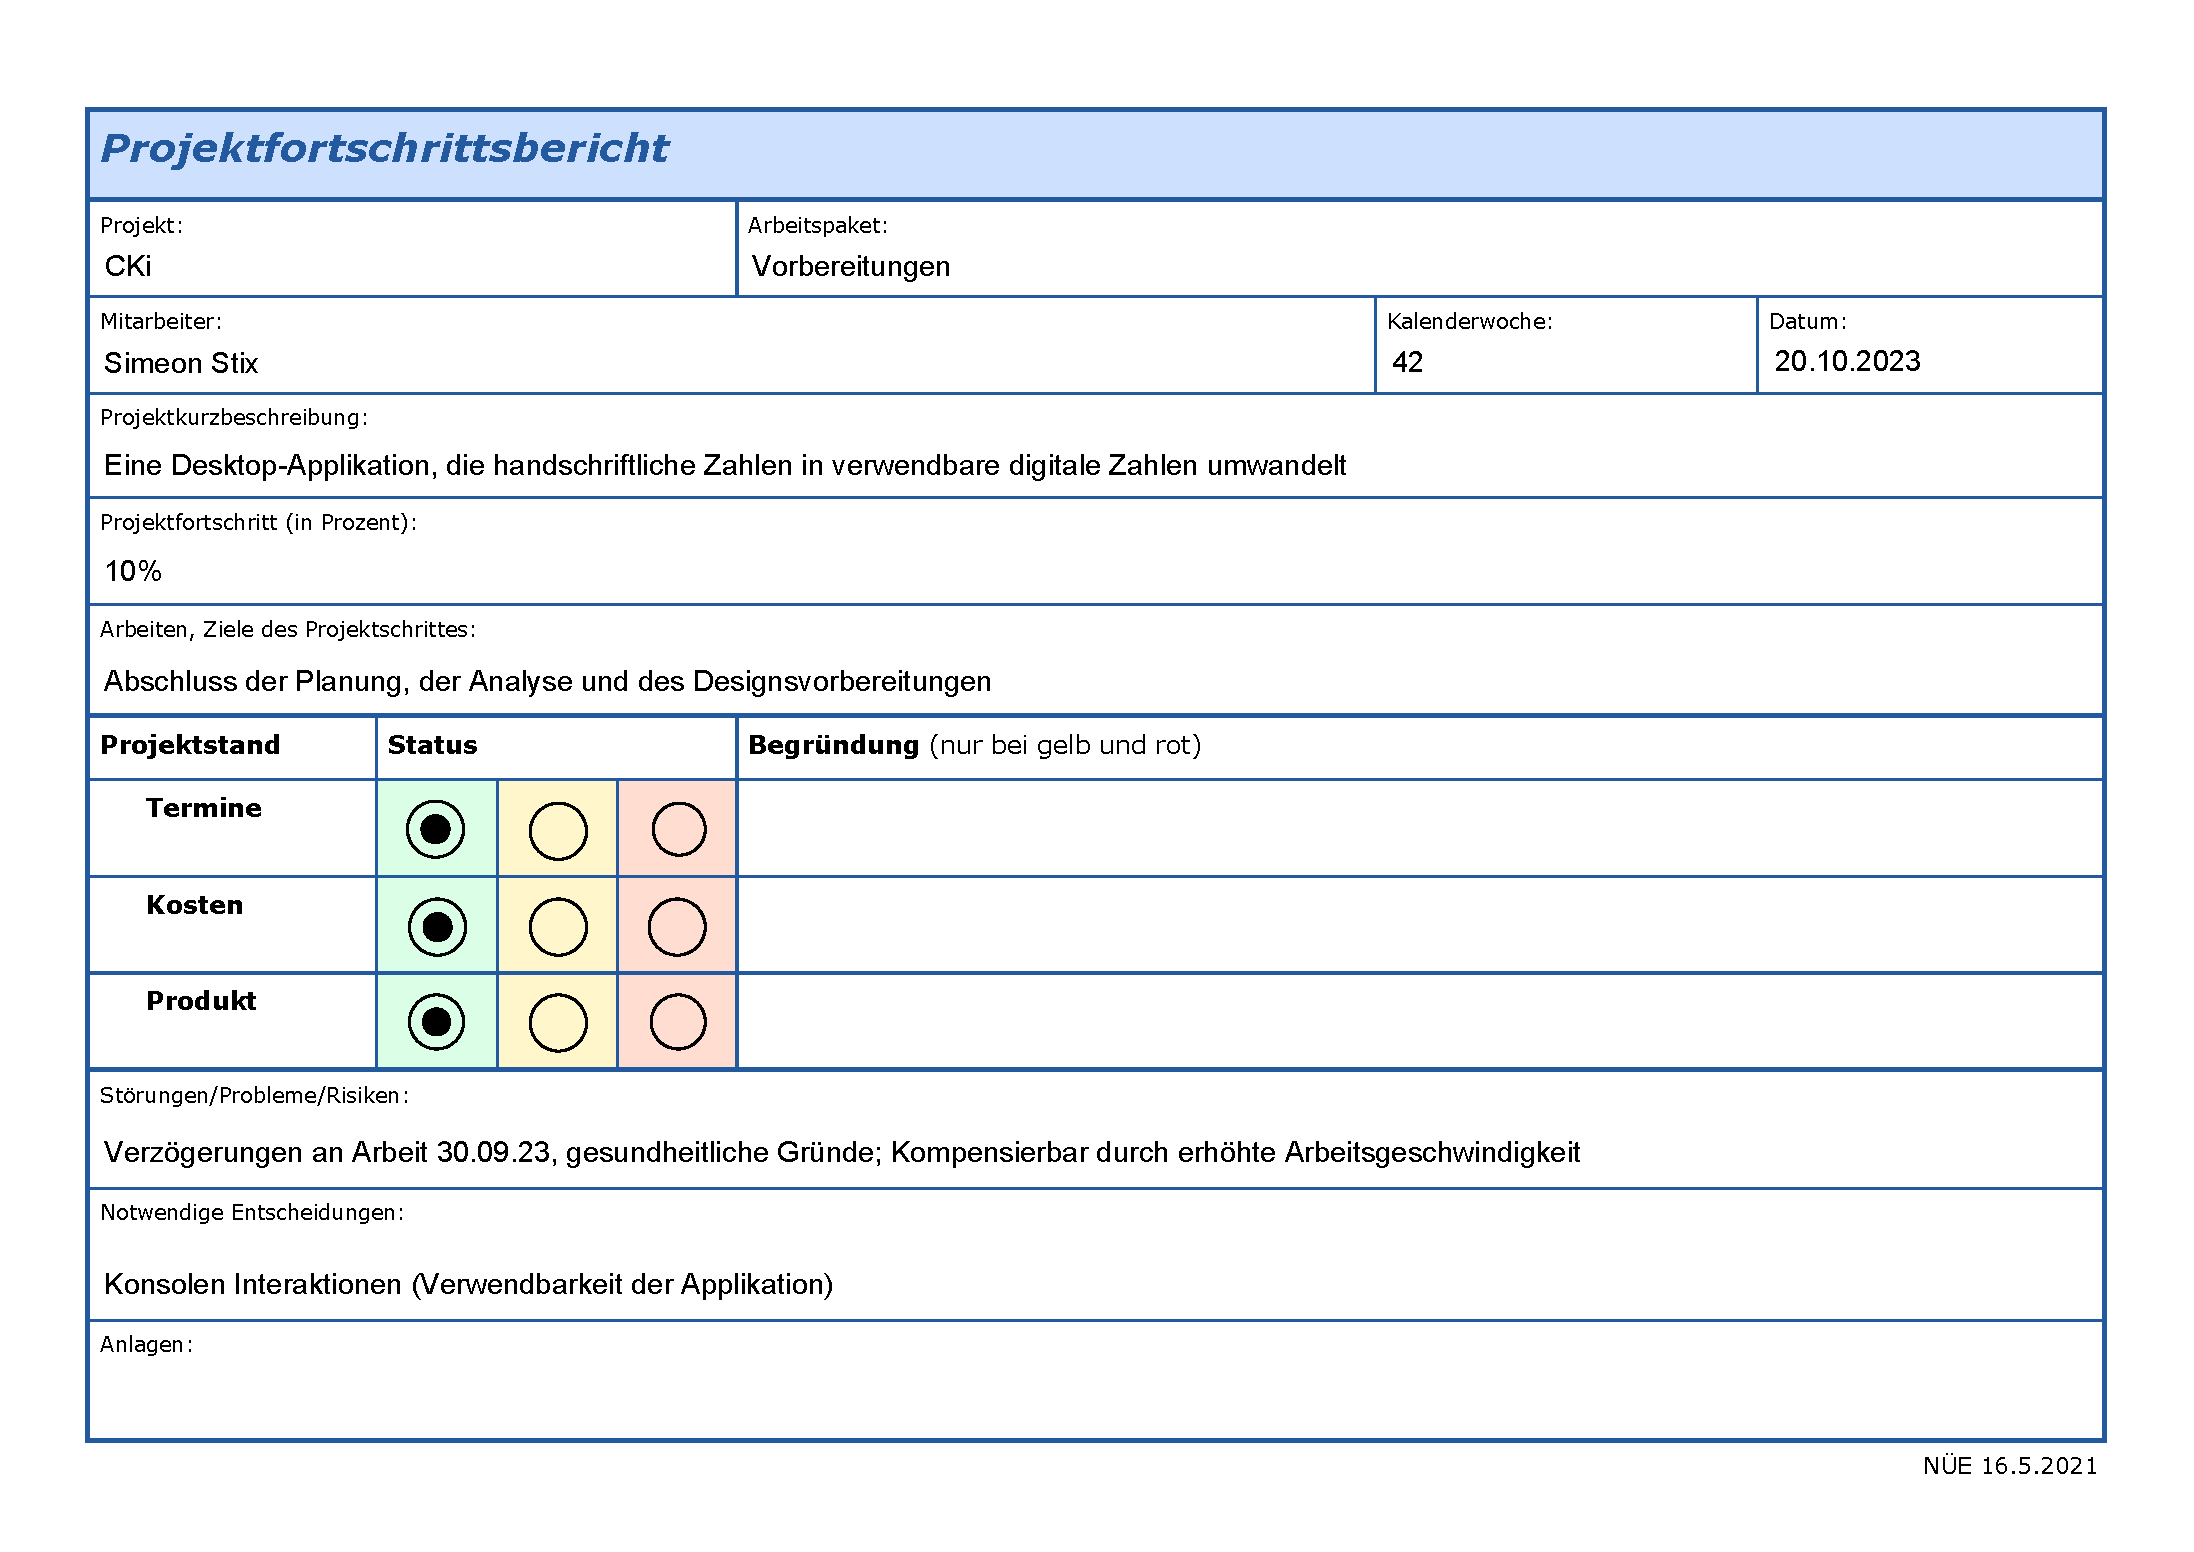
\includepdf[pages=-]{./appendix/Fortschrittsbericht_01_Stix_2023-10-20.pdf}
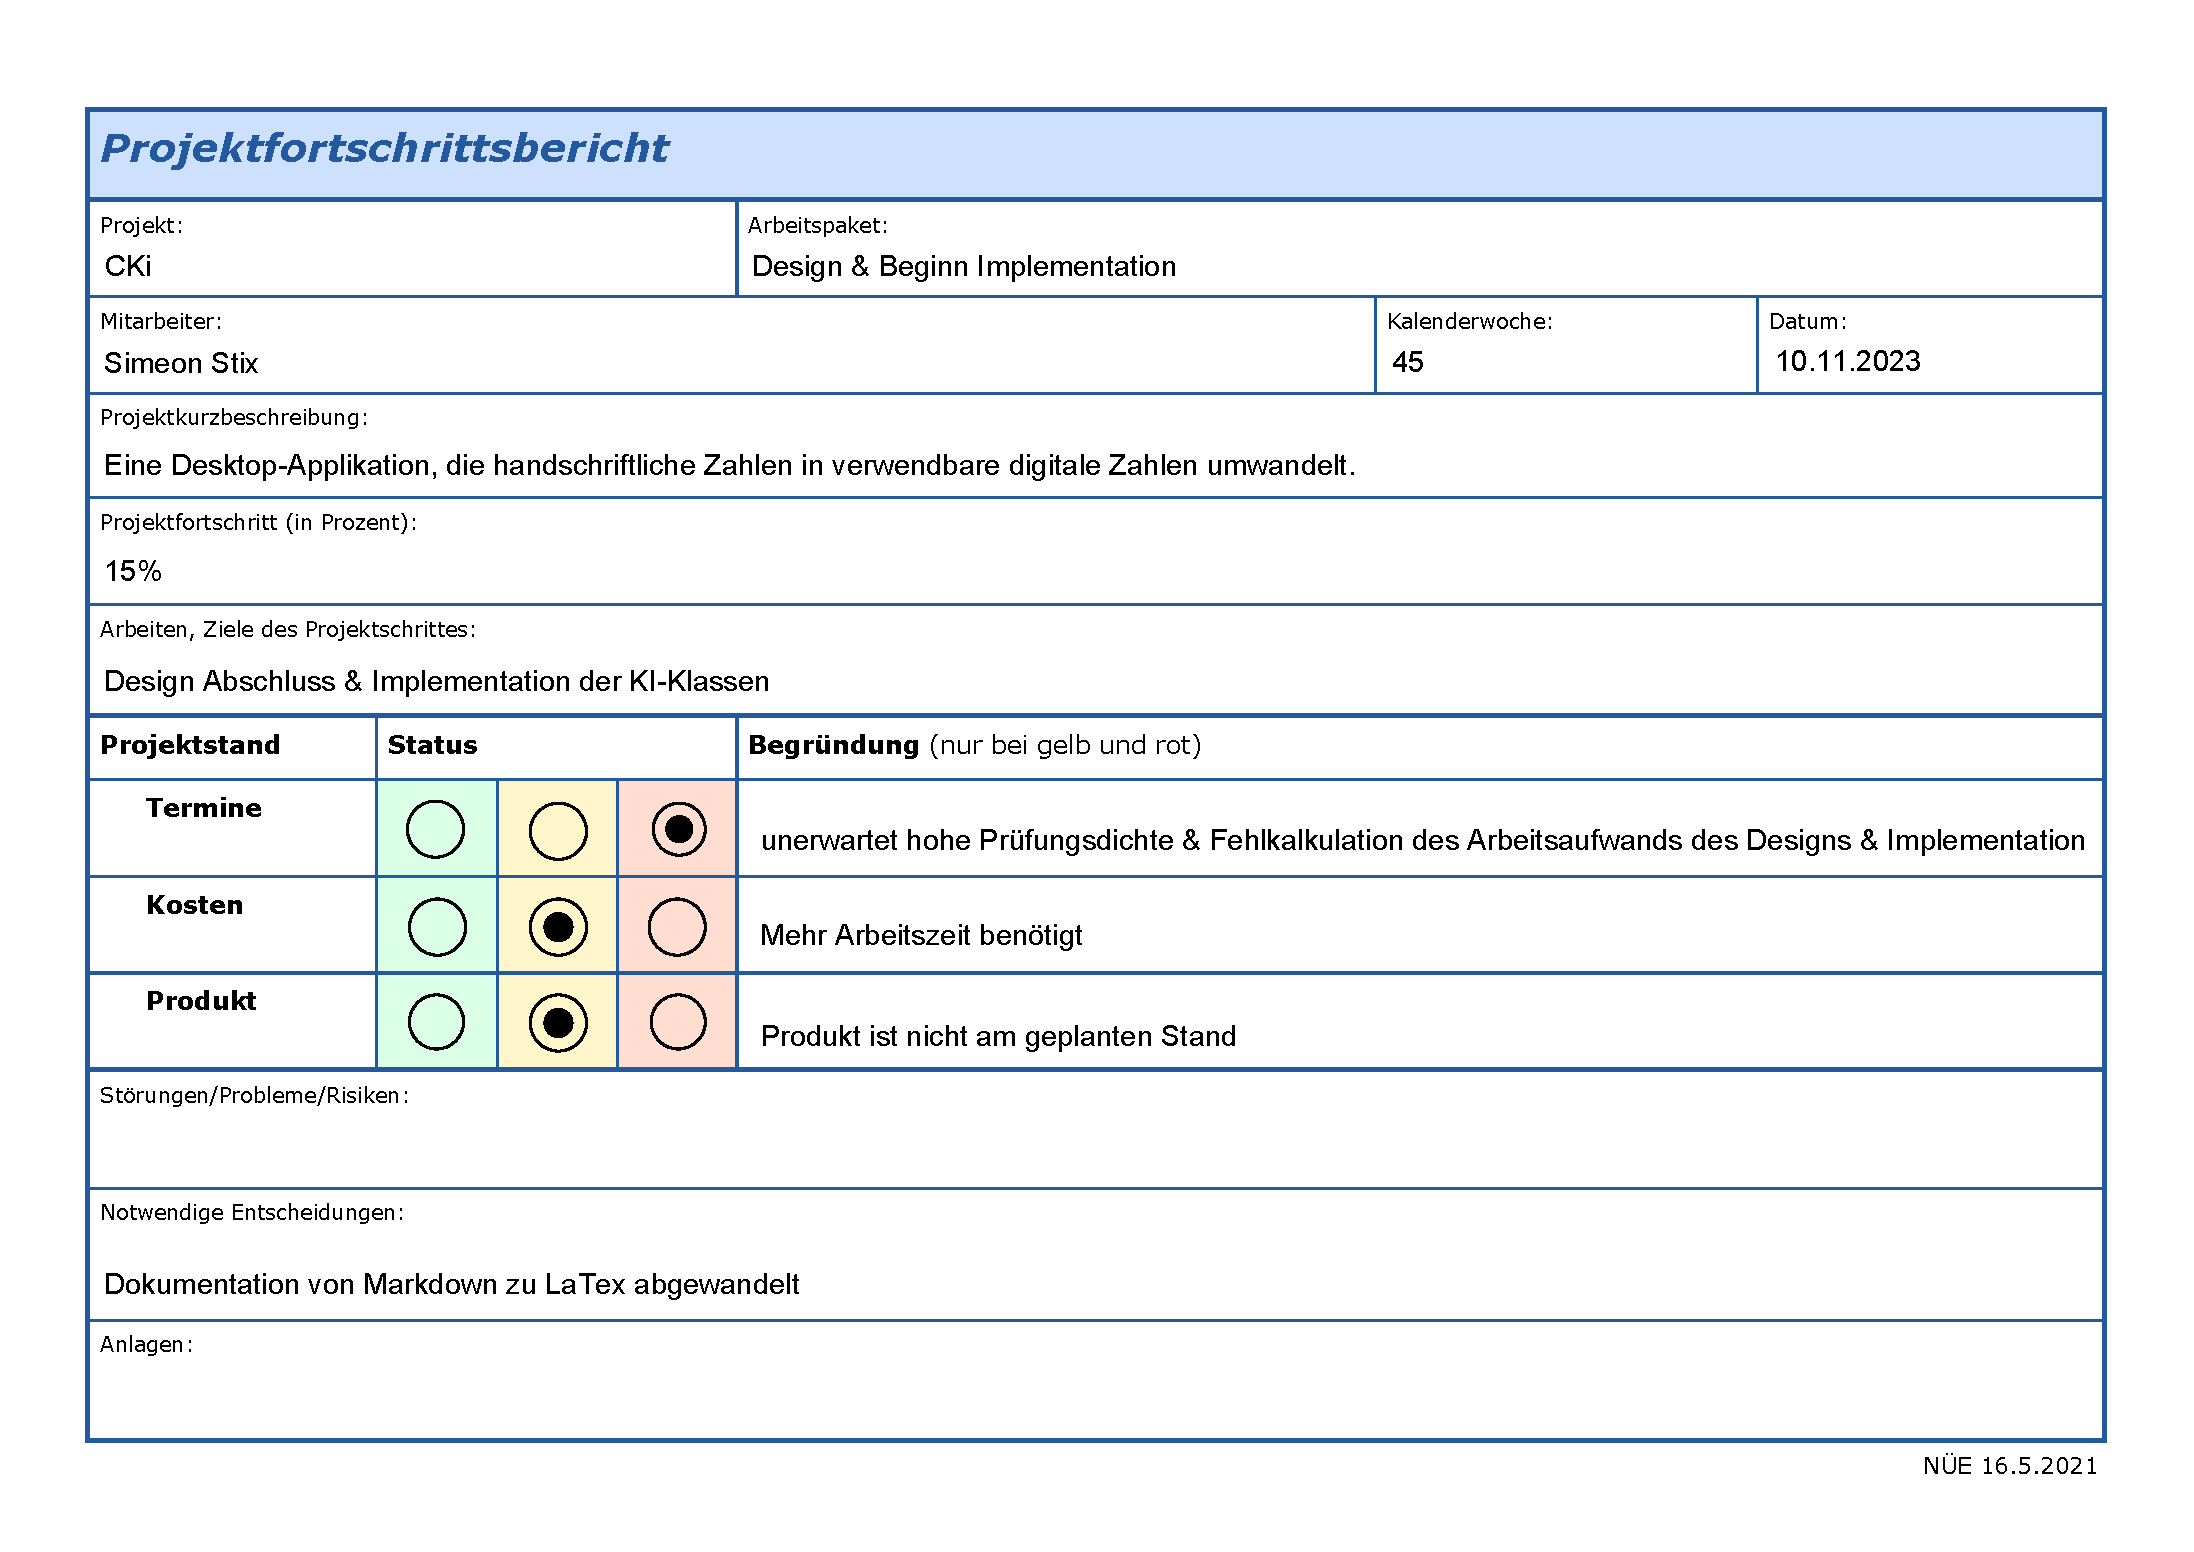
\includepdf[pages=-]{./appendix/Fortschrittsbericht_02_Stix_2023-11-10.pdf}
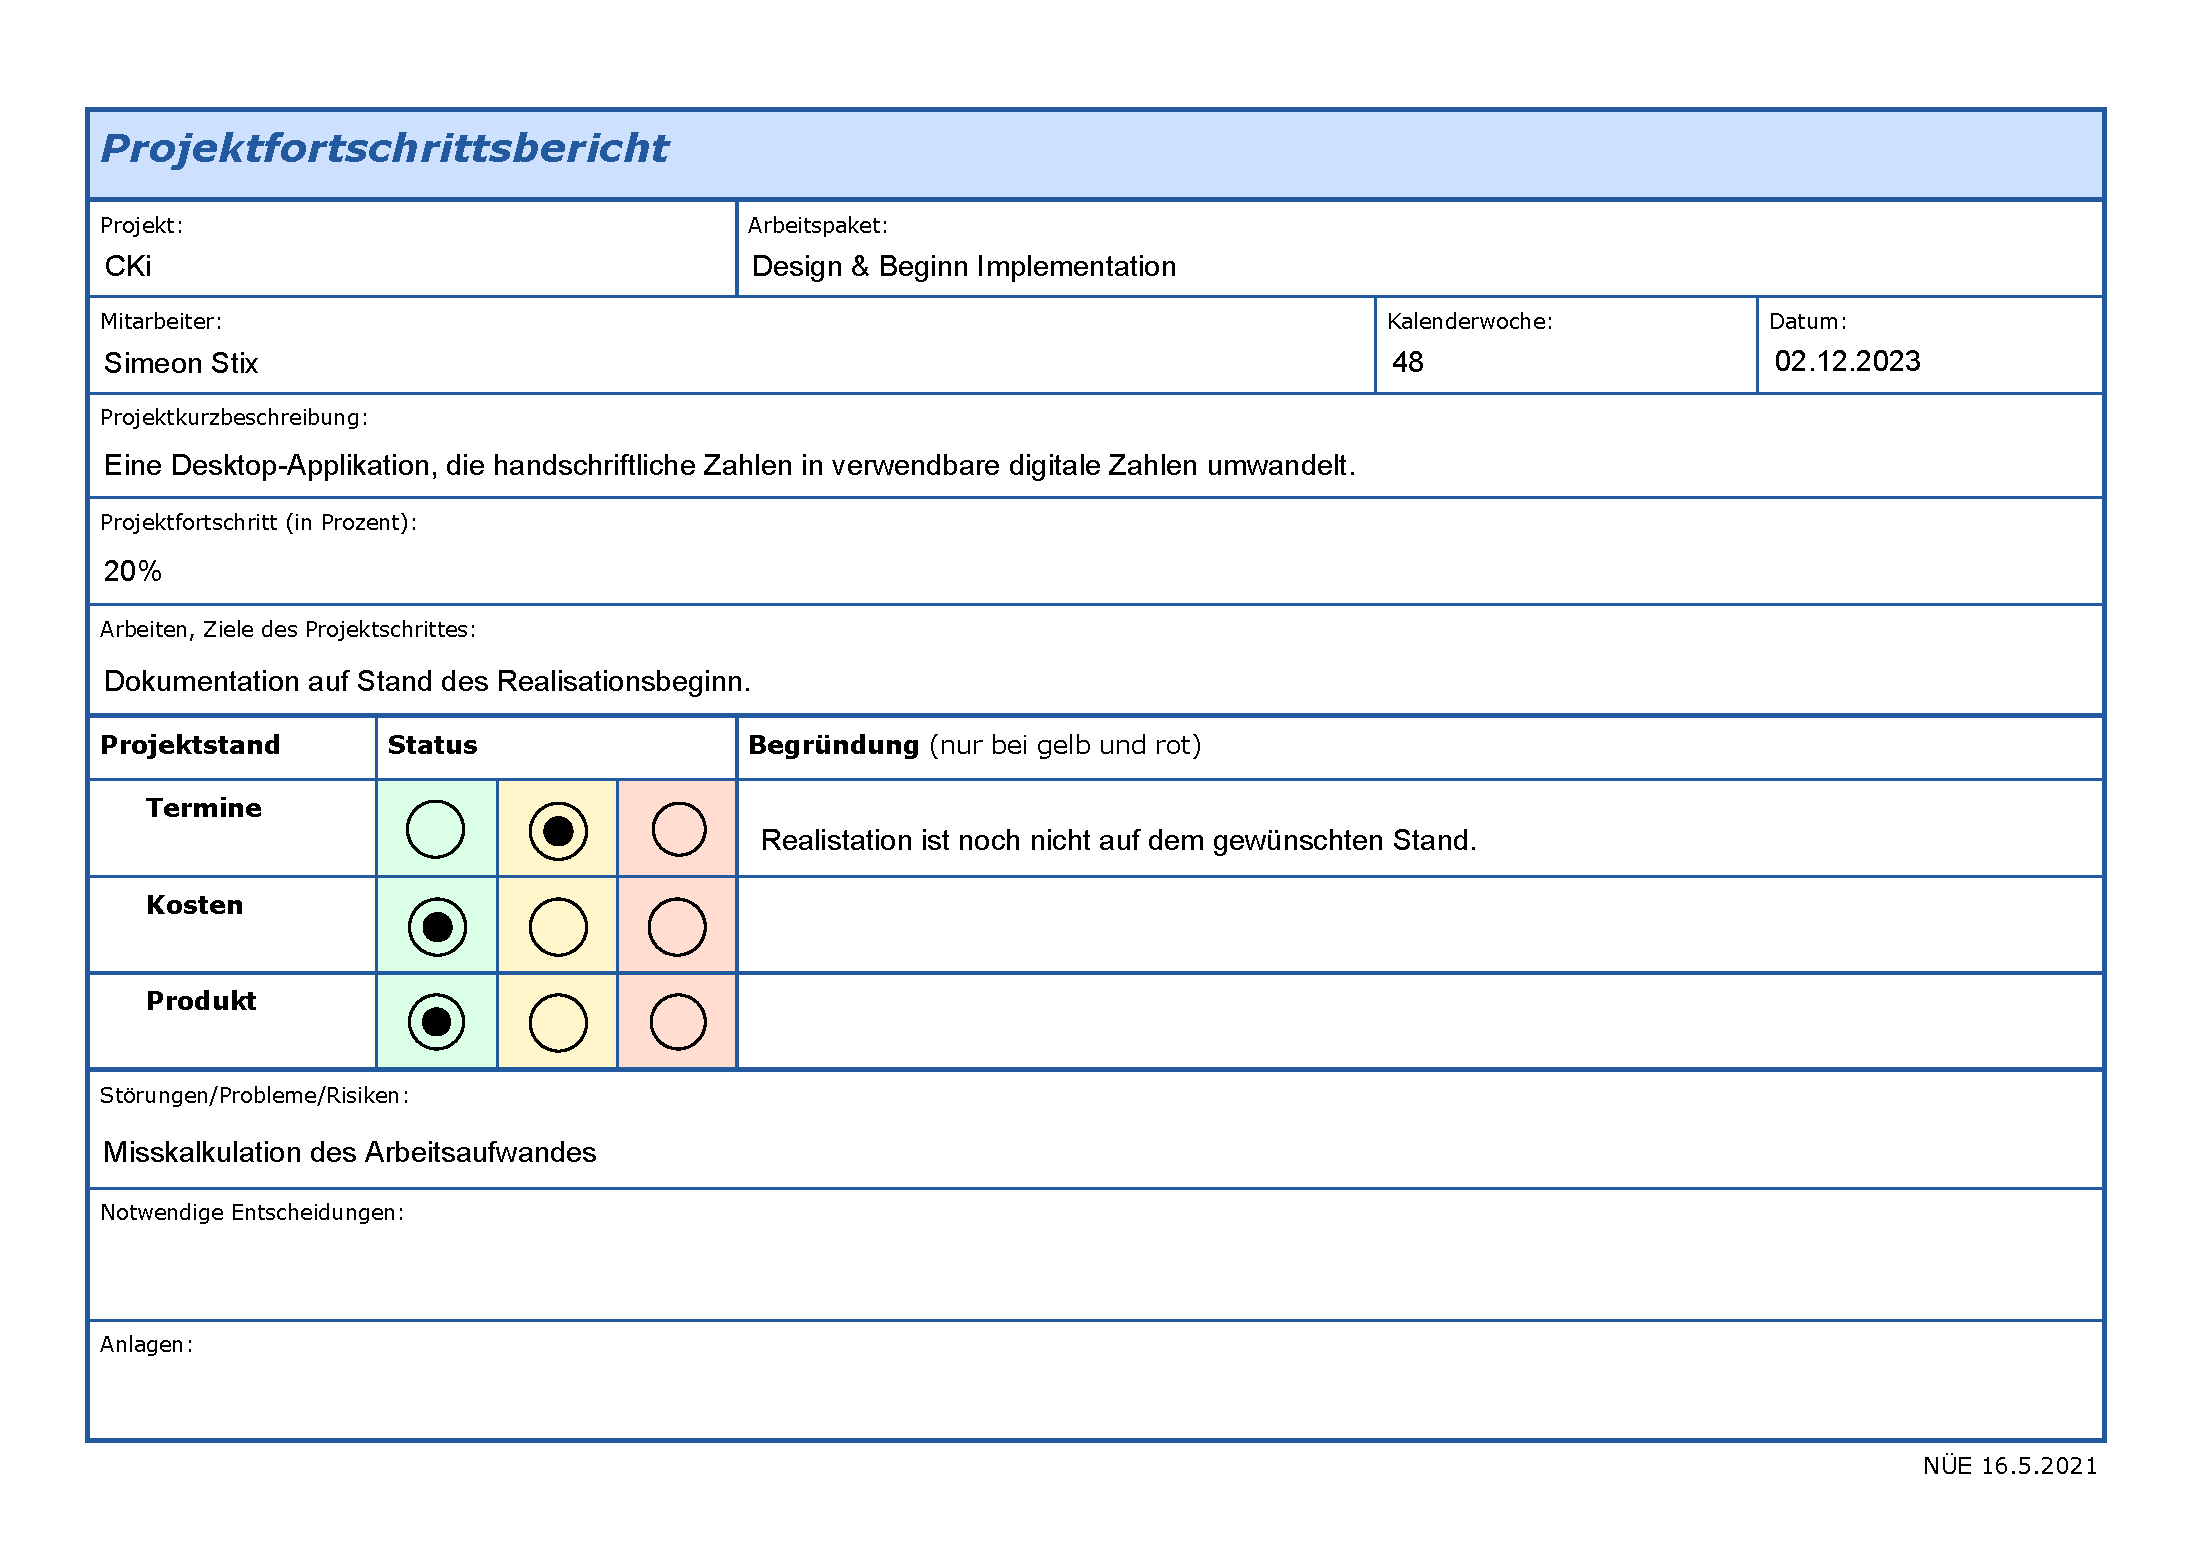
\includepdf[pages=-]{./appendix/Fortschrittsbericht_03_Stix_2023-12-02.pdf}
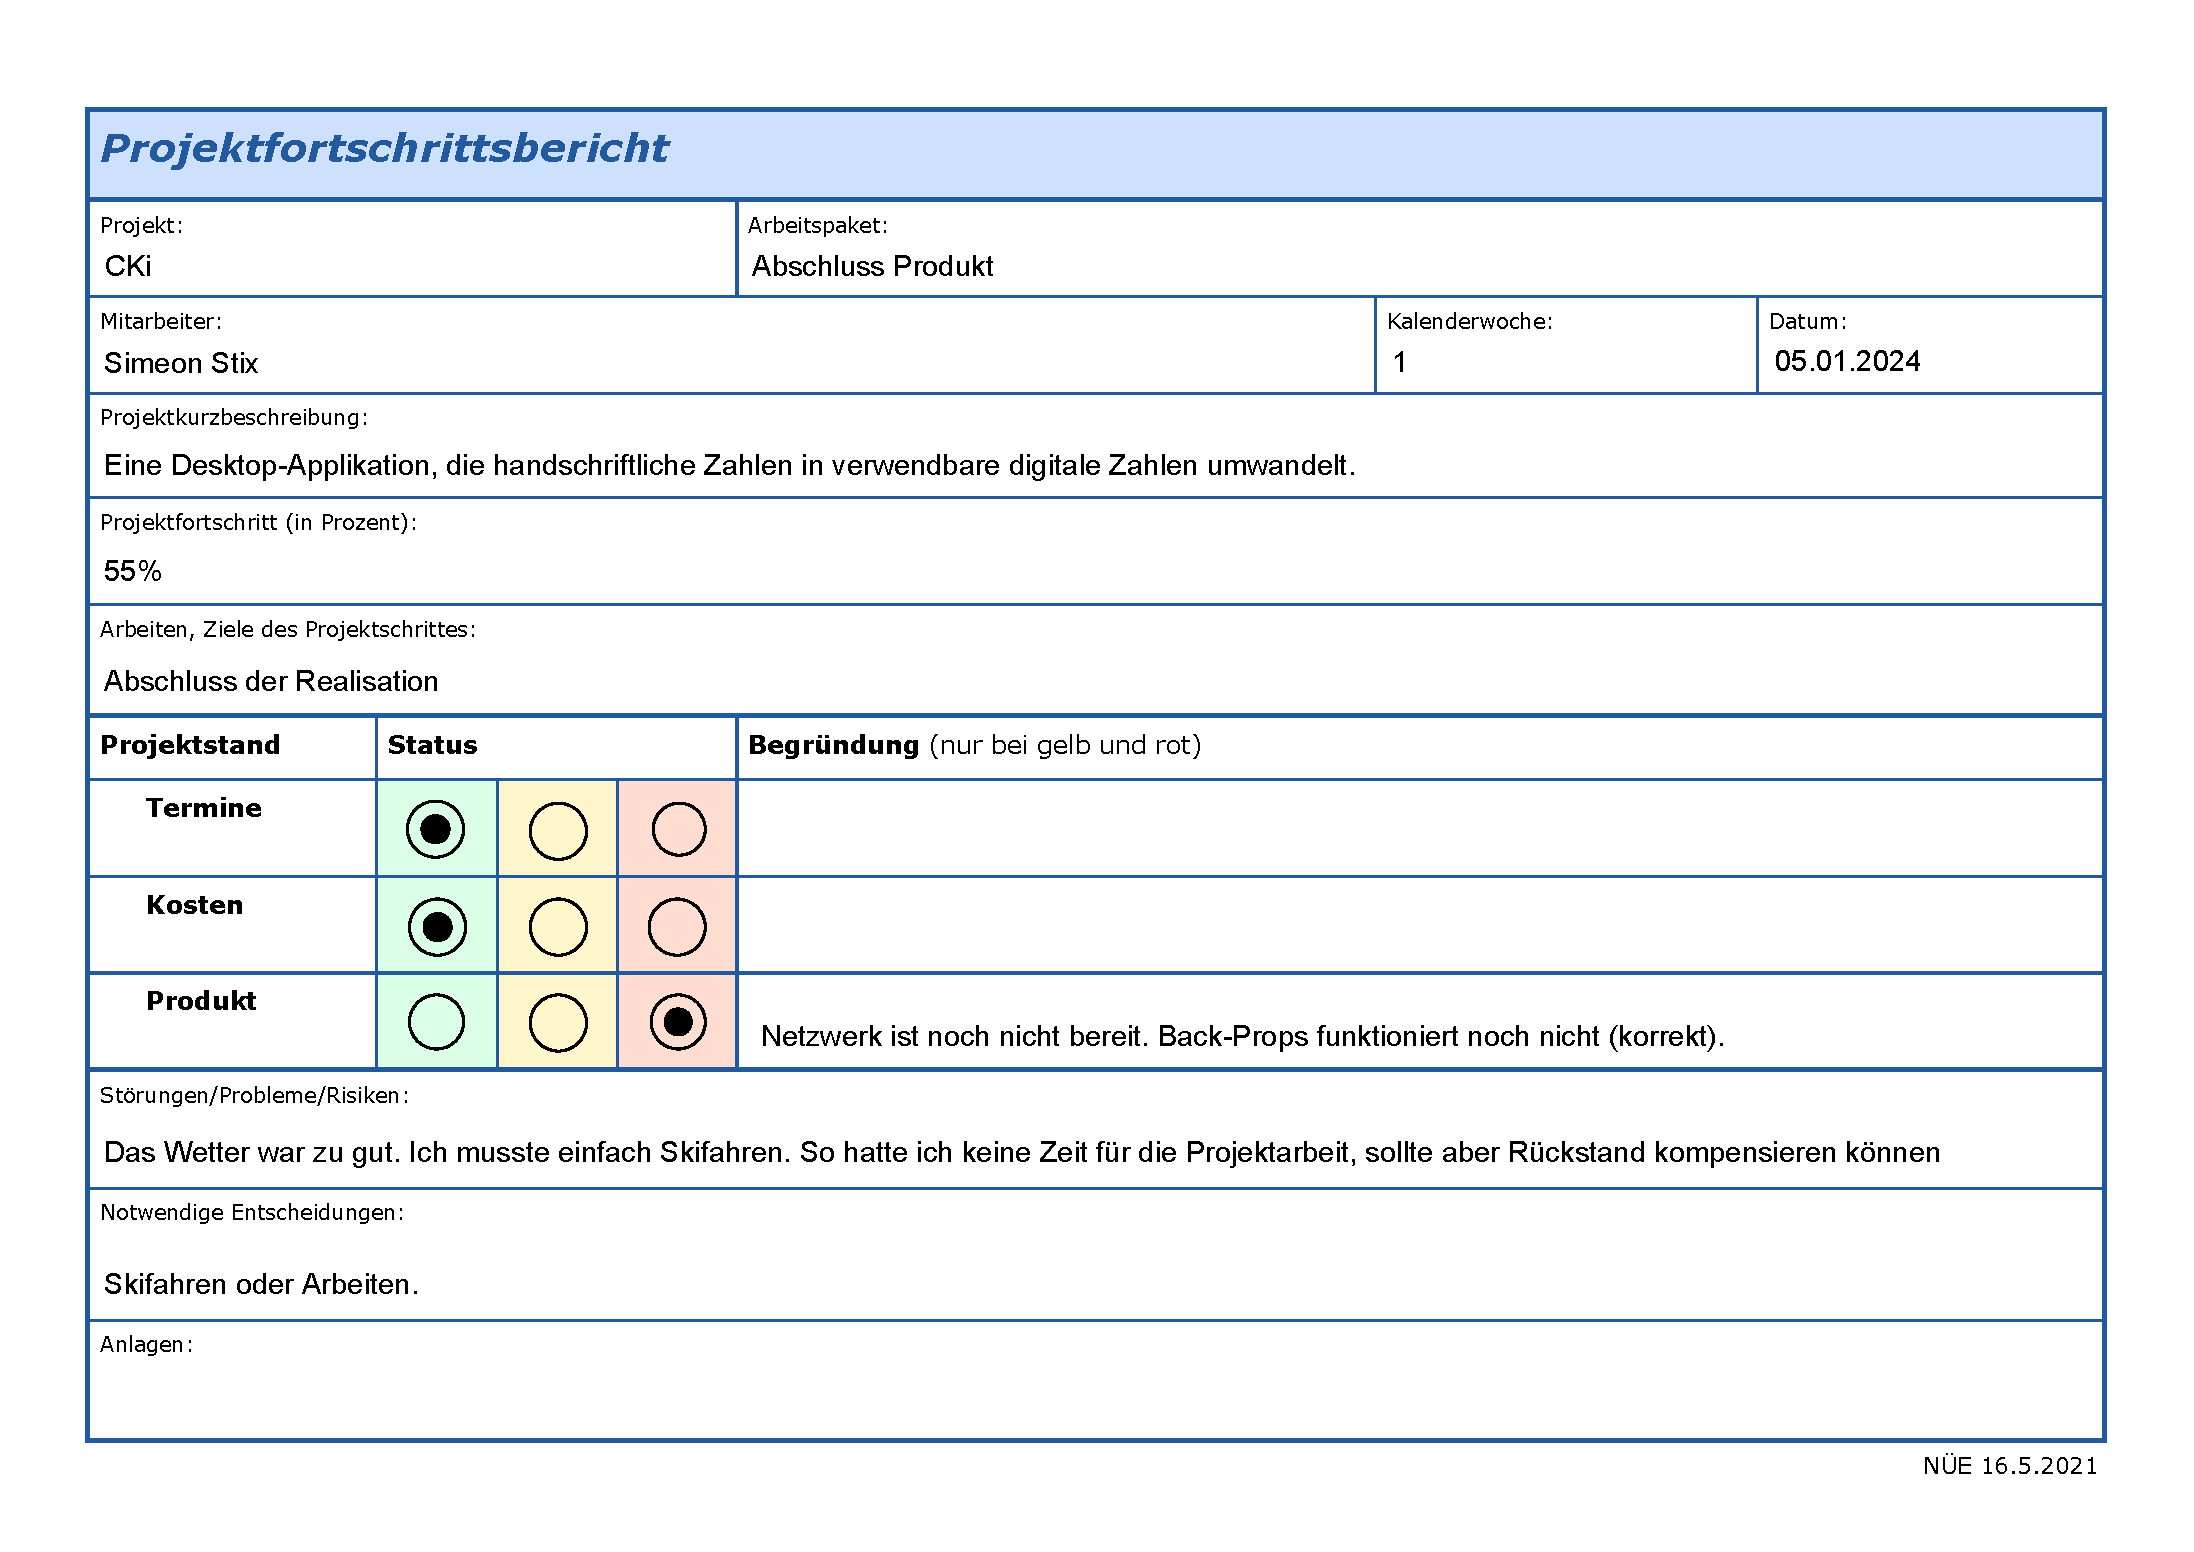
\includepdf[pages=-]{./appendix/Fortschrittsbericht_04_Stix_2024-01-05.pdf}
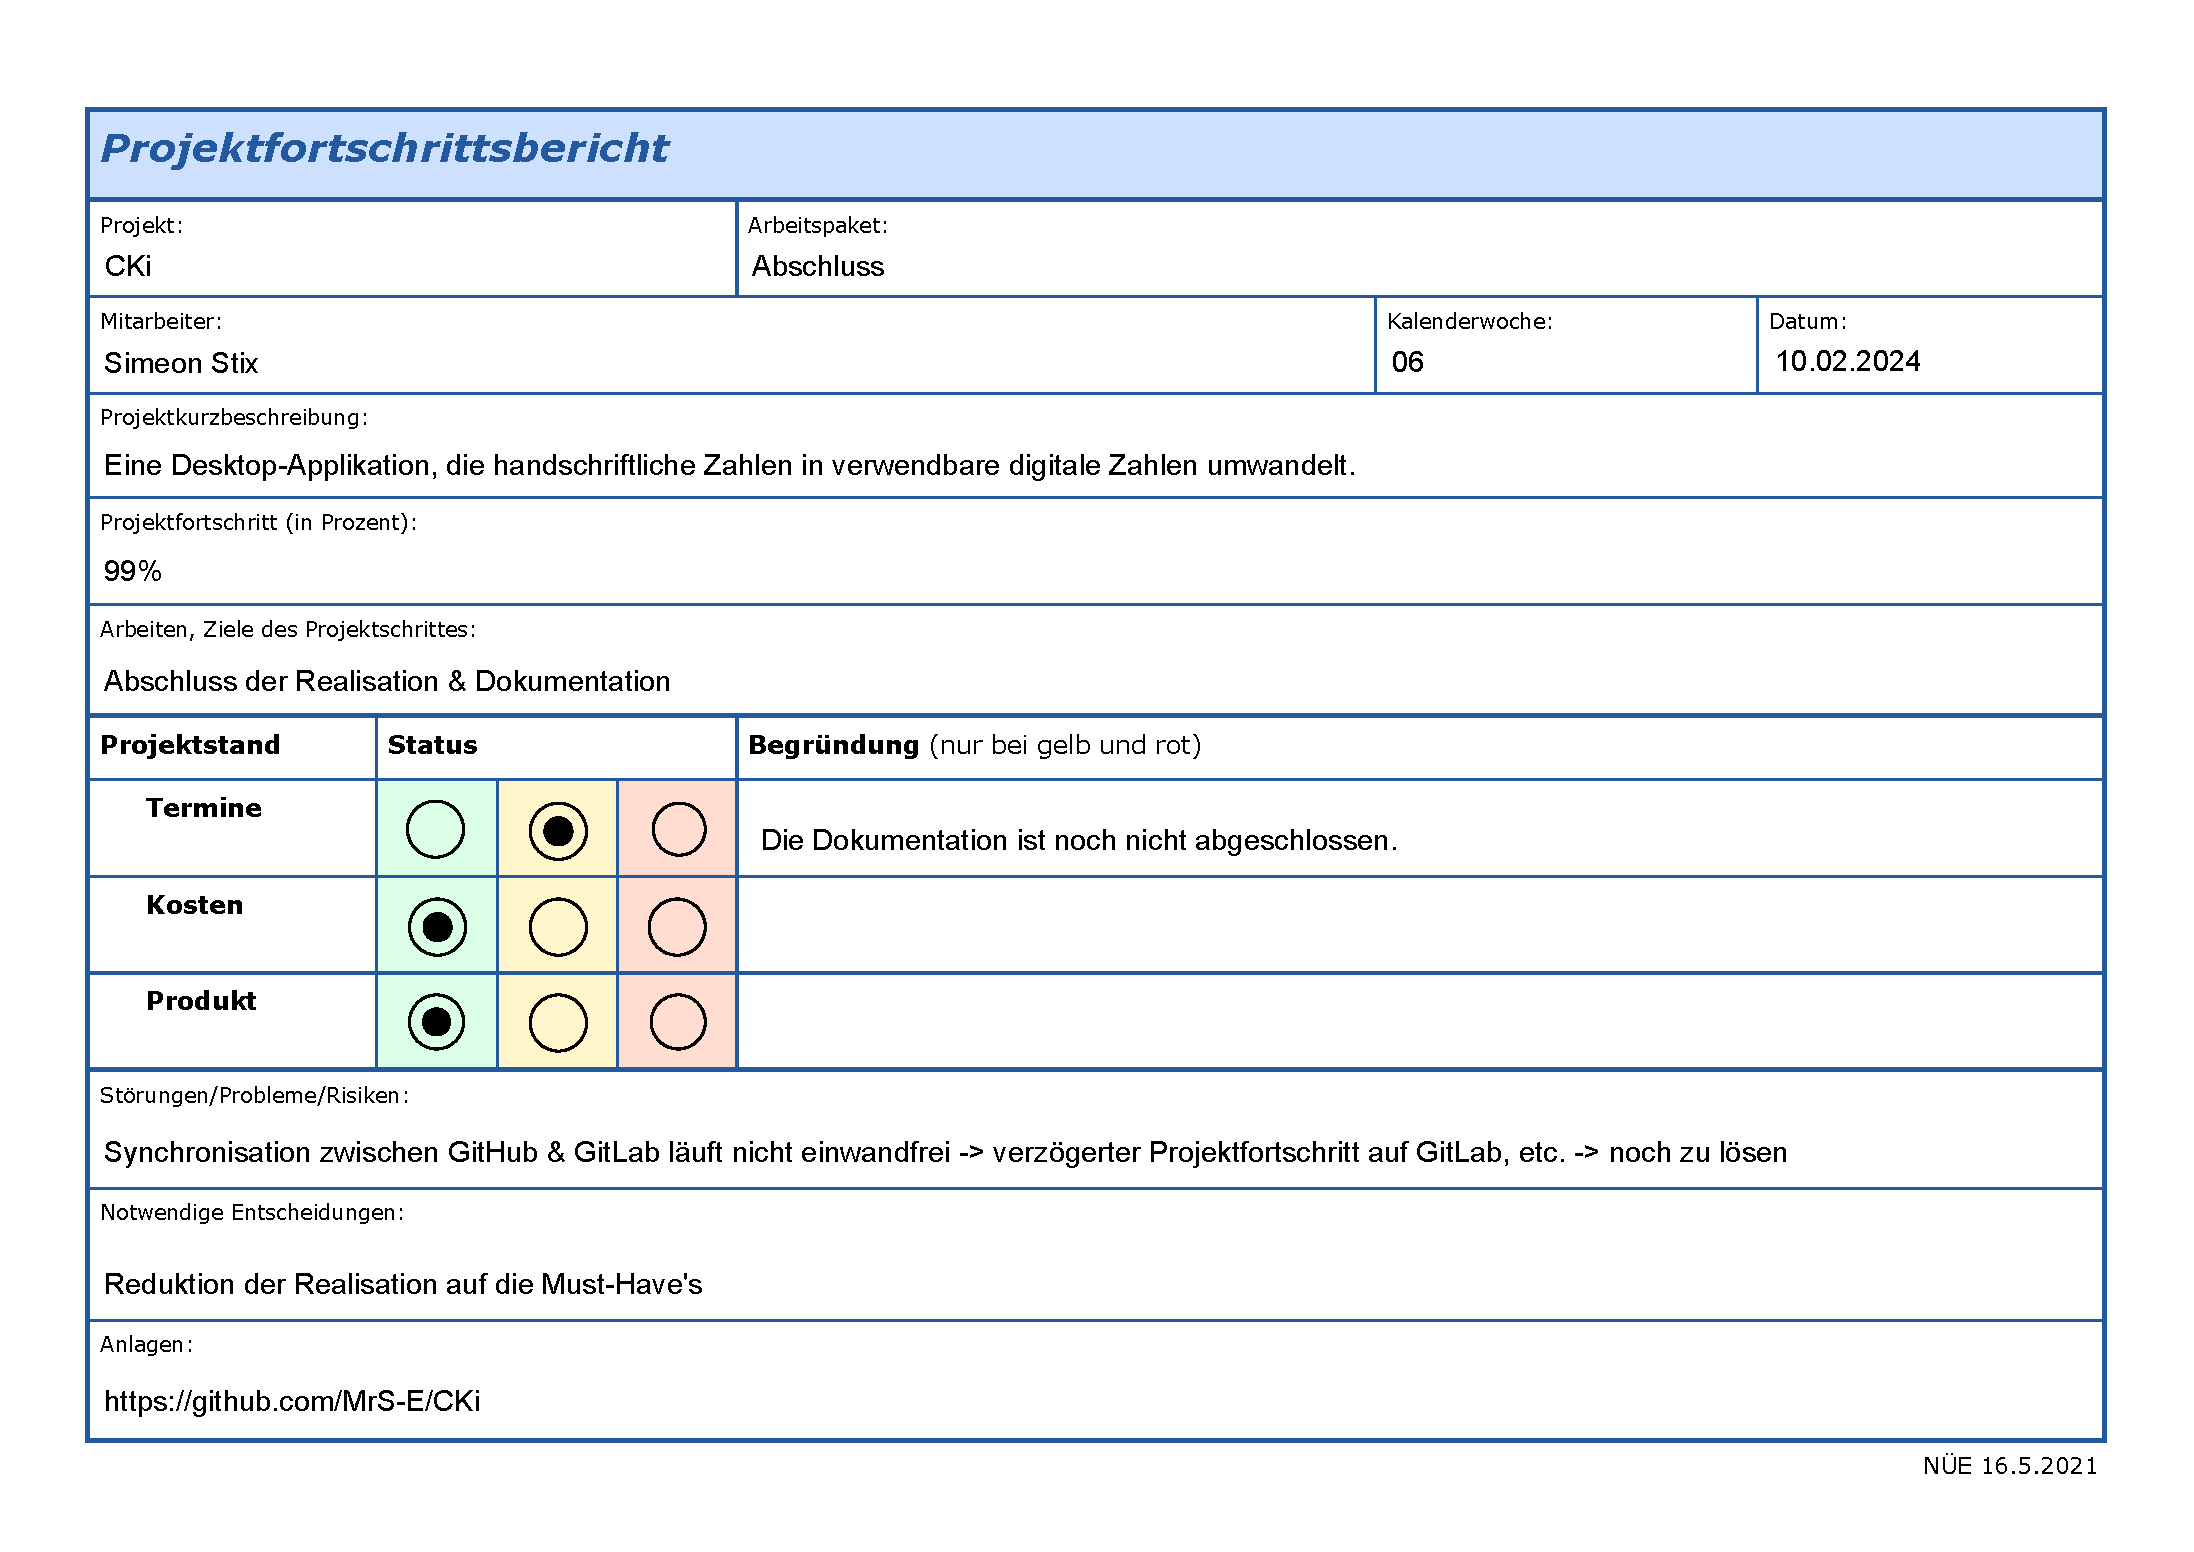
\includepdf[pages=-]{./appendix/Fortschrittsbericht_05_Stix_2024-02-10.pdf}
\end{appendices}

\end{document}

